\documentclass[conference]{IEEEtran}

% --- Tiếng Việt và Bảng mã ---
\usepackage[utf8]{inputenc}
\usepackage[T5]{fontenc}

% --- Thư viện cần thiết ---
\usepackage{cite}
\usepackage{amsmath,amssymb,amsfonts}
\usepackage{graphicx}
\usepackage{booktabs}
\usepackage{microtype}
\usepackage{dblfloatfix}
\usepackage{url}
\usepackage{array}
\usepackage{titlesec}
\usepackage{enumitem}
\usepackage[skip=4pt, font=footnotesize]{caption}

% --- Cấu hình phân bố float (Hình ảnh và Bảng) ---
\setcounter{topnumber}{4}
\setcounter{bottomnumber}{3}
\setcounter{totalnumber}{8}
\renewcommand{\topfraction}{0.95}
\renewcommand{\bottomfraction}{0.85}
\renewcommand{\textfraction}{0.08}
\renewcommand{\floatpagefraction}{0.80}
\renewcommand{\dbltopfraction}{0.95}
\renewcommand{\dblfloatpagefraction}{0.80}

\setlength{\textfloatsep}{7pt plus 2pt minus 1pt}
\setlength{\floatsep}{6pt plus 2pt minus 1pt}
\setlength{\intextsep}{6pt plus 2pt minus 1pt}

% --- Khoảng cách tiêu đề các mục ---
\titlespacing*{\section}{0pt}{6.5pt plus 1.5pt minus 1.0pt}{3.5pt plus 1.0pt minus 1.0pt}
\titlespacing*{\subsection}{0pt}{5.0pt plus 1.0pt minus 1.0pt}{2.5pt plus 0.8pt minus 0.8pt}
\titlespacing*{\subsubsection}{0pt}{3.5pt plus 0.8pt minus 0.8pt}{2.0pt plus 0.5pt minus 0.5pt}

\setlist{nosep, leftmargin=1.3em}

\begin{document}

\title{Thiết Kế Hệ Thống Vi Mạch SoC AI Biên Mini-PULP Tích Hợp Bộ Tăng Tốc Xấp Xỉ Logarit Zero-DSP Cho Nhận Dạng Chữ Số Thời Gian Thực}

\author{
    \IEEEauthorblockN{Nguyễn Văn Thực, Lê Nhật Minh}
    \IEEEauthorblockA{Khoa Điện - Điện tử, Trường Đại học Sư phạm Kỹ thuật TP. Hồ Chí Minh (HCMUTE)\\
    Email: 24161421@student.hcmute.edu.vn}
}

\maketitle

\begin{abstract}
Nghiên cứu đề xuất và hiện thực hóa hệ thống vi mạch SoC AI biên Mini-PULP tích hợp bộ tăng tốc phần cứng tự trị LA-HWPE phục vụ nhận dạng chữ số viết tay MNIST thời gian thực trên FPGA AMD Xilinx Zynq-7000 (\texttt{xc7z010clg400-1}). Hệ thống kết hợp lõi điều khiển 32-bit RISC-V RV32I, hệ thống bus thanh ghi CSR phân xử phi khóa, bộ nhớ đa ngân hàng TCDM 34.6~KB trên chip và mảng tính toán $1\times 4$ SIMD sử dụng mạch nhân xấp xỉ logarit đột phá hoàn toàn không tiêu tốn khối nhân DSP. Nhờ chuẩn nén trọng số Log8 8-bit trên bus chuẩn 32-bit (giải phóng 10 khối BRAM36), bộ mã hóa bit 1 (LOD) dùng chung và kỹ thuật đường ống hóa vi kiến trúc MAC 2 tầng sâu, thiết kế đạt chuẩn ký kết định thời vật lý tại xung nhịp 100.0~MHz với độ dôi thời gian thiết lập WNS đạt $+1.392\text{ ns}$ ($F_{\max} = 116.17\text{ MHz}$). Kết quả sau đặt và định tuyến vật lý trên AMD Vivado 2024.2 ghi nhận toàn bộ SoC chỉ tiêu tốn 2,931 Slice LUTs (16.65\%), 2,252 Flip-Flops (6.40\%), 18 Block RAMs (30.00\%) và 0 DSP48E1 (0.00\%). Tại 100~MHz, hệ thống đạt độ trễ suy luận $127.96\,\mu\text{s}$/ảnh (7,815 FPS), công suất động 59.0~mW và năng lượng suy luận siêu thấp $7.55\,\mu\text{J}$/ảnh với độ chính xác đạt 93.88\% trên 10,000 ảnh kiểm thử MNIST, mang lại giải pháp tối ưu cho các hệ thống nhúng biên năng lượng cực thấp.
\end{abstract}

\begin{IEEEkeywords}
Edge AI SoC, Mini-PULP, Zero-DSP Accelerator, Logarithmic Computing, RISC-V RV32I, TinyML, FPGA Physical Sign-Off, Center-of-Mass Preprocessing, MNIST Real-Time.
\end{IEEEkeywords}

\section{Đặt Vấn Đề và Động Lực Thiết Kế}
\label{sec:intro}

\subsection{Bối Cảnh Trí Tuệ Nhân Tạo Biên và Thách Thức Khan Hiếm Tài Nguyên}
\hspace*{1em} Trong kỷ nguyên bùng nổ của Internet vạn vật và trí tuệ nhân tạo biên, nhu cầu triển khai các mô hình mạng nơ-ron học sâu trực tiếp trên các vi điều khiển và thiết bị nhúng năng lượng thấp ngày càng trở nên cấp bách. Việc suy luận trực tiếp tại biên mang lại nhiều ưu điểm vượt trội: loại bỏ hoàn toàn độ trễ truyền dẫn mạng lên máy chủ đám mây, bảo toàn quyền riêng tư của dữ liệu người dùng, nâng cao tính an ninh và đảm bảo khả năng hoạt động độc lập ngay cả khi mất kết nối mạng.

Tuy nhiên, các mô hình học sâu hiện đại, dù là mạng nơ-ron đa tầng hay mạng nơ-ron tích chập, đều đòi hỏi khối lượng phép tính số học khổng lồ, đặc biệt là các phép nhân tích lũy MAC. Trên các nền tảng phần cứng nhúng và vi mạch FPGA cỡ nhỏ như AMD Xilinx Zynq-7000 (\texttt{xc7z010-1}), số lượng khối nhân phần cứng chuyên dụng DSP48E1 bị giới hạn nghiêm ngặt ở mức vỏn vẹn 80 khối. Việc sử dụng các lõi nhân số học chính xác 16-bit hoặc 32-bit thông thường để thực thi hàng trăm nghìn phép tính MAC dẫn đến ba điểm nghẽn vật lý PPA cốt tử:
\begin{enumerate}
    \item \textbf{Cạn kiệt tài nguyên khối DSP:} Một bộ tăng tốc AI truyền thống nếu mở rộng số lượng PE song song sẽ nhanh chóng chiếm dụng hết 80 khối DSP48E1, khiến chip không còn tài nguyên cho các khối giao tiếp ngoại vi, xử lý tín hiệu hình ảnh, âm thanh hoặc mở rộng chức năng SoC.
    \item \textbf{Tiêu hao công suất động và tỏa nhiệt lớn:} Các khối nhân mảng cộng tích riêng có mật độ chuyển mạch tín hiệu rất cao, gây sụt áp trên đường nguồn nội $V_{\text{CCINT}}$ và làm tăng công suất động vượt quá ngân sách cho phép của các thiết bị pin và nguồn năng lượng thấp.
    \item \textbf{Điểm nghẽn định thời đường truyền tổ hợp:} Đường truyền số học dài từ đầu vào trọng số, qua bộ nhân, tới bộ cộng tích lũy 32-bit tạo nên đường trễ tổ hợp lên tới $11 - 14\text{ ns}$, kéo tần số hoạt động của chip xuống dưới 80~MHz, gây suy giảm nghiêm ngặt thông lượng xử lý.
\end{enumerate}

\subsection{Cảm Hứng Từ Kiến Trúc PULP và Động Lực Thiết Kế}
\hspace*{1em} Nhằm giải quyết triệt để bài toán hóc búa trên, nghiên cứu này lấy cảm hứng từ nền tảng điện toán siêu tiết kiệm năng lượng song song PULP do Đại học ETH Zurich và Đại học Bologna tiên phong phát triển \cite{pulp2019, conti2015}. Kiến trúc PULP nổi tiếng với triết lý phân tách rành mạch giữa điều khiển và tính toán:
\begin{itemize}
    \item \textbf{Mặt bằng điều khiển trung tâm (Host Control Plane):} Sử dụng vi xử lý mở RISC-V làm lõi điều phối thông minh, xử lý các tác vụ quản lý luồng dữ liệu, cấu hình thanh ghi ngoại vi và truyền thông UART \cite{waterman2014}.
    \item \textbf{Mặt bằng dữ liệu tính toán (Data Plane):} Sử dụng bộ tăng tốc phần cứng tự trị chuyên dụng LA-HWPE để thực thi các khối tính toán ma trận với hiệu suất cao nhất trên từng miliwatt công suất \cite{conti2015}.
    \item \textbf{Bộ nhớ dữ liệu ghép nối chặt (TCDM):} Bộ nhớ SRAM trên chip chia sẻ đa ngân hàng không xung đột, triệt tiêu hoàn toàn nhu cầu truy xuất bộ nhớ DDR ngoài vốn tiêu tốn năng lượng gấp $100 - 1,000$ lần so với truy xuất on-chip.
\end{itemize}

Kết hợp triết lý PULP với tính kháng lỗi nội tại của các mạng nơ-ron nhân tạo, nghiên cứu đề xuất một kiến trúc bộ tăng tốc xấp xỉ logarit đột phá: chuyển đổi toàn bộ miền tính toán nhân sang miền cộng logarit nhị phân \cite{mitchell1962, guo2021}. Bằng cách loại bỏ hoàn toàn các khối nhân số học DSP48E1 và nén trọng số theo định dạng Log8 8-bit trên bus 32-bit, hệ thống đạt được hiệu năng năng lượng vượt bậc mà vẫn giữ vững độ chính xác phân loại tương đương mô hình toán học chuẩn trên tập dữ liệu chuẩn MNIST \cite{lecun1998}.

\subsection{Các Đóng Góp Nổi Bật của Công Trình}
\hspace*{1em} Công trình nghiên cứu mang lại 5 đóng góp học thuật và kỹ thuật cốt lõi:
\begin{enumerate}
    \item \textbf{Kiến trúc Mini-PULP Edge AI SoC Hoàn Chỉnh:} Hiện thực hóa vi mạch SoC tích hợp hoàn chỉnh trên FPGA gồm lõi CPU 32-bit RISC-V RV32I tối ưu hóa chốt thanh ghi giải mã, phân hệ tăng tốc tự trị LA-HWPE, hệ thống bus điều khiển CSR và bộ nhớ đa ngân hàng TCDM 34.6~KB độc lập.
    \item \textbf{Mạch Nhân Xấp Xỉ Logarit Zero-DSP Đột Phá:} Đề xuất vi kiến trúc nhân logarit tách kênh định trị kết hợp hiệu chỉnh vi bảng tra $\text{LUT}_8$, triệt tiêu hoàn toàn mảng cộng tích riêng và giải phóng 100\% tài nguyên khối cứng DSP ($\text{DSP} = 0/80$, $0.00\%$).
    \item \textbf{Chuẩn Nén Trọng Số Log8 \& Bus Chuẩn 32-bit:} Sáng tạo định dạng mã hóa Log8 8-bit $\{s, k[2:0], m[3:0]\}$ cho trọng số tĩnh với cơ chế giải nén trực tiếp tại PE MAC, thu hẹp bề rộng bus từ 48-bit xuống đúng 32-bit chuẩn SoC, cắt giảm 10 khối BRAM36 (-41.7\% dung lượng BRAM trọng số) mà không làm suy giảm độ chính xác.
    \item \textbf{Đường Ống Hóa Sâu 2 Tầng và Ký Kết Định Thời An Toàn 100 MHz:} Tách rời đường trễ $11.61\text{ ns}$ thành 2 tầng đường ống độc lập $\le 4.5\text{ ns}$, kết hợp bộ tìm cực đại Argmax dạng cây nhị phân song song 2 tầng, đạt chuẩn ký kết vật lý an toàn tại 100~MHz ($\text{WNS} = +1.392\text{ ns}$, $F_{\max} = 116.17\text{ MHz}$).
    \item \textbf{Thuật Toán Tiền Xử Lý Căn Tâm Khối Lượng và Hệ Thống Live Demo:} Xây dựng thuật toán căn tâm khối lượng giải quyết triệt để hiện tượng lệch góc khi vẽ tay, tích hợp cùng máy chủ Web GUI trực quan thời gian thực hỗ trợ đồng thời chế độ mô phỏng vi mạch chu kỳ chính xác và kit phần cứng vật lý qua UART.
\end{enumerate}

\section{Cơ Sở Lý Thuyết Số Học Logarit và Chuẩn Nén Trọng Số Log8}
\label{sec:theory_log8}

\subsection{Thuật Toán Số Học Logarit Mitchell và Phân Tích Sai Số}
\hspace*{1em} Thuật toán số học logarit xấp xỉ cổ điển Mitchell \cite{mitchell1962} dựa trên việc xấp xỉ hàm logarit nhị phân $\log_2(1 + x) \approx x$ với $x \in [0, 1)$. Một số nguyên không dấu 8-bit $a \in [0, 255]$ được biểu diễn dưới dạng dấu phẩy động nhị phân chuẩn hóa:
\begin{equation}
    a = 2^{k_a}(1 + x_a), \quad k_a = \lfloor \log_2 a \rfloor \in [0, 7], \quad x_a \in [0, 1)
    \label{eq:mitchell_decomp}
\end{equation}
trong đó $k_a$ là số nguyên chỉ vị trí của bit 1 cao nhất thu được qua khối phát hiện bit 1 (LOD), và $x_a$ là phần định trị.

Khi đó, logarit cơ số 2 của hai số $a$ và $b$ được xấp xỉ tuyến tính:
\begin{equation}
    \log_2(a \cdot b) = \log_2 a + \log_2 b \approx (k_a + k_b) + (x_a + x_b)
\end{equation}
Phép nhân hai số được chuyển đổi thành phép cộng trong miền logarit, sau đó lấy hàm nghịch đảo logarit bằng cách dịch bit:
\begin{equation}
    a \cdot b \approx 
    \begin{cases}
        2^{k_a + k_b}(1 + x_a + x_b), & \text{khi } x_a + x_b < 1 \\
        2^{k_a + k_b + 1}(x_a + x_b), & \text{khi } x_a + x_b \ge 1
    \end{cases}
\end{equation}

Mặc dù thuật toán Mitchell thuần túy loại bỏ được phép nhân, sai số xấp xỉ tương đối của nó khá lớn, với sai số phi tuyến lồi cực đại đạt tới $E_{\max} \approx 0.08607$ ($8.61\%$). Khi tích lũy qua hàng nghìn lượt nhân-cộng trong mạng nơ-ron học sâu, sai số này gây suy giảm nghiêm trọng độ chính xác phân lớp.

\subsection{Số Học Logarit Tách Kênh Không Bộ Cộng}
\hspace*{1em} Để khắc phục triệt để sai số của thuật toán Mitchell mà không làm phát sinh trễ số học từ bộ cộng lan truyền mượn nhớ, nghiên cứu đề xuất kỹ thuật phân tách kênh định trị kết hợp vi bảng tra \cite{guo2021}:
\begin{equation}
    x_a[5:0] \longrightarrow \{ x_H[2:0],\, x_L[2:0] \}
\end{equation}
trong đó 6-bit định trị được chia thành 3-bit trọng số cao $x_H = x_a[5:3]$ đóng vai trò xấp xỉ thô và 3-bit trọng số thấp $x_L = x_a[2:0]$ đóng vai trò hiệu chỉnh tinh.

Bảng tra vi mô 8 phần tử ($\text{LUT}_8$) được thiết kế tối ưu toán học để bù đắp chính xác độ cong phi tuyến của hàm logarit:
\begin{equation}
    \text{LUT}_8 = [1, 3, 4, 4, 6, 6, 7, 7]
\end{equation}
Từ mã logarit 9-bit hoàn chỉnh được tạo nên bằng cơ chế ghép nối bus trực tiếp không qua bộ cộng:
\begin{equation}
    \text{Log}(a) = \{ k_a[2:0],\, x_H[2:0],\, \text{LUT}_8[x_L][2:0] \}
    \label{eq:log_concat}
\end{equation}
Cơ chế ghép bus~(\ref{eq:log_concat}) chỉ sử dụng dây dẫn và logic bảng tra vi mô $\text{LUT}_8$, tiêu tốn đúng 0 cổng cộng logic và 0 trễ số học, tạo ra từ mã 9-bit trung thực với sai số trung bình giảm xuống dưới $1.32\%$.

\subsection{Chuẩn Nén Trọng Số Tiền Mã Hóa Thu Gọn Log8}
\hspace*{1em} Trong các bài toán suy luận tại biên, trọng số mạng $W \in [-128, 127]$ đã được huấn luyện cố định và không thay đổi trong suốt quá trình vận hành. Ở phiên bản thiết kế v0.2.0 trước đây, mỗi trọng số logarit được mã hóa thành 12-bit đóng gói $\{ \text{sign}, \text{zero}, \text{Log}(|W|)[8:0] \}$. Để cung cấp song song cho 4 PE trong mảng SIMD $1\times 4$, bus dữ liệu từ BRAM bắt buộc phải có độ rộng 48-bit ($4 \times 12$-bit). Độ rộng 48-bit này gây lãng phí bộ nhớ Block RAM do cấu trúc BRAM36 hỗ trợ tối ưu ở cấu hình 32-bit hoặc 64-bit, làm tiêu tốn tới 24 khối RAMB36 chỉ riêng cho phần trọng số.

Để tối ưu hóa toàn diện PPA, kiến trúc v0.3.0 sáng tạo chuẩn nén Log8: Mỗi trọng số tĩnh được lượng tử hóa và nén vừa khít trong đúng 1 byte (8-bit), với cấu trúc trường bit:
\begin{equation}
    \text{Code}_{\text{Log8}}[7:0] = \{ s,\, k[2:0],\, m[3:0] \}
\end{equation}
trong đó:
\begin{itemize}
    \item $s = \text{Code}[7]$: Bit dấu (1 ứng với số âm, 0 ứng với số dương).
    \item $k[2:0] = \text{Code}[6:4]$: Số mũ nguyên nhị phân $k \in [0, 6]$ biểu thị bậc độ lớn $2^k$.
    \item $m[3:0] = \text{Code}[3:0]$: Định trị thu gọn 4-bit $m \in [0, 15]$.
    \item \textbf{Mã dự trữ số không ($W = 0$):} Do trọng số có $|W| \le 127$ nên số mũ $k$ tối đa chỉ là 6 ($2^6 = 64 \le 127$). Số mũ $k = 7$ hoàn toàn không thể xuất hiện trong dải giá trị thực. Do đó, mã nhị phân \texttt{0x7F} ($\{s=0, k=7, m=15\}$) được dành riêng để đại diện cho giá trị $W = 0$.
\end{itemize}

\subsection{Cơ Chế Giải Nén Trực Tiếp Tại Phần Tử Xử Lý}
\hspace*{1em} Khi nạp từ BRAM vào mảng tính toán, từ mã Log8 8-bit được giải nén trực tiếp thành từ mã logarit 9-bit bên trong từng PE bằng phương pháp nhân bản bit cao:
\begin{equation}
    \text{frac}_6 = \{ m[3:0],\, m[3:2] \}
\end{equation}
\begin{equation}
    \text{weight\_log}[8:0] = \{ k[2:0],\, \text{frac}_6[5:0] \}
\end{equation}
\begin{equation}
    \text{weight\_sign} = \text{Code}[7], \quad \text{weight\_zero} = (\text{Code} == \texttt{8'h7F})
\end{equation}

Nhờ phép ghép nối thuần túy này, phần cứng giải nén trong PE tiêu tốn 0 cổng logic và 0 trễ phát sinh, trong khi bus trọng số được thu hẹp về đúng 32-bit ($4 \times 8$-bit), hoàn toàn tương thích với bus dữ liệu chuẩn của SoC RISC-V. Dung lượng BRAM lưu trữ trọng số giảm từ 49.2~KB xuống 32.8~KB, giải phóng ngay lập tức 10 khối RAMB36 (-41.7\% dung lượng BRAM trọng số).

\subsection{Hàm Lượng Tử Hóa Hợp Nhất}
\hspace*{1em} Kết quả tích lũy 32-bit của nơ-ron tầng ẩn sau khi cộng bias được nén ngược về biểu diễn INT8 có dấu phục vụ tầng tiếp theo thông qua hàm lượng tử hóa hợp nhất:
\begin{equation}
    \text{Requant}(y) = \text{clamp}\left( \lfloor (y + 2^{\text{SHIFT}-1}) \gg \text{SHIFT} \rfloor,\, 0,\, 127 \right)
\end{equation}
với hệ số dịch bit chuẩn hóa $\text{SHIFT} = 11$. Hàm triệt tiêu hoàn toàn các giá trị âm (tích hợp hàm kích hoạt phi tuyến ReLU) và ghim dải bão hòa không dấu trong $[0, 127]$, đảm bảo dải động số học luôn ổn định không bị tràn bit.

% ==============================================================================
% MỤC III: KIẾN TRÚC VI MẠCH TỔNG THỂ SOC - HÌNH 1 (FULL-WIDTH)
% ==============================================================================
\section{Kiến Trúc Vi Mạch Tổng Thể Hệ Thống Mini-PULP SoC}
\label{sec:soc_arch}

\begin{figure*}[!t]
    \centering
    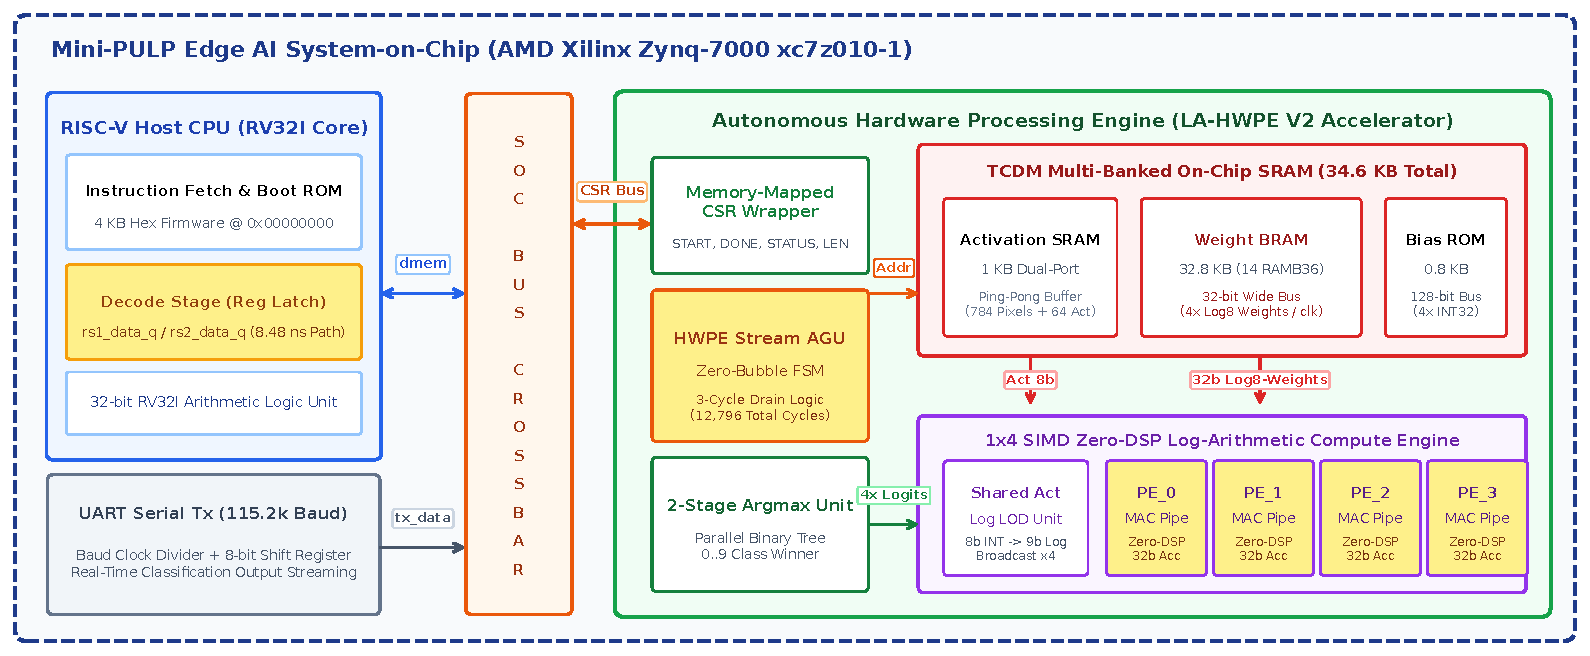
\includegraphics[width=0.98\textwidth]{figures/fig_soc_arch.pdf}
    \caption{Sơ đồ khối vi kiến trúc hoàn chỉnh của hệ thống vi mạch Mini-PULP Edge AI SoC: Tích hợp Host CPU RISC-V RV32I, bus điều khiển Interconnect, bộ truyền nối tiếp UART, hệ thống bộ nhớ đa ngân hàng TCDM 34.6 KB (16 khối RAMB36E1) và bộ tăng tốc tự trị LA-HWPE với mảng tính toán $1\times 4$ SIMD Zero-DSP.}
    \label{fig:soc_arch}
\end{figure*}

\subsection{Tổng Quan Hệ Thống và Phân Tách Miền Hoạt Động}
\hspace*{1em} Kiến trúc phần cứng tổng thể của Mini-PULP Edge AI SoC được minh họa chi tiết trên Hình~\ref{fig:soc_arch}. Hệ thống được phân tách một cách rành mạch thành hai miền chức năng:
\begin{itemize}
    \item \textbf{Host Control Plane:} Đảm nhiệm vai trò quản lý hệ thống, thực thi firmware điều khiển, thiết lập cấu hình mạng, phân phối tín hiệu kích hoạt và điều phối giao tiếp UART với thiết bị ngoài.
    \item \textbf{Data Plane:} Gồm bộ tăng tốc phần cứng tự trị LA-HWPE và hệ thống bộ nhớ đa ngân hàng TCDM, trực tiếp xử lý các luồng tính toán ma trận thông lượng lớn mà không làm tiêu tốn chu kỳ lệnh của CPU.
\end{itemize}

\subsection{Host Control Plane: Lõi Vi Điều Khiển RISC-V RV32I Nhúng}
\hspace*{1em} Lõi vi xử lý RISC-V 32-bit RV32I nguyên bản được thiết kế theo kiến trúc máy trạng thái hữu hạn tối ưu cho môi trường FPGA nhúng \cite{waterman2014}. CPU thực thi tập lệnh cơ sở số nguyên RV32I từ bộ nhớ Boot ROM 4~KB tích hợp tại địa chỉ \texttt{0x00000000}. 

Để đạt được tần số hoạt động cao trên fabric FPGA Xilinx Zynq, vi kiến trúc CPU được áp dụng cơ chế chốt thanh ghi giải mã:
\begin{itemize}
    \item Tại trạng thái giải mã lệnh \texttt{STATE\_DECODE}, dữ liệu đọc từ mảng thanh ghi đa dụng 32 thanh ghi (\texttt{regfile[rs1]}, \texttt{regfile[rs2]}) được chốt trực tiếp vào hai thanh ghi trung gian \texttt{rs1\_data\_q} và \texttt{rs2\_data\_q}.
    \item Cơ chế chốt này cắt rời hoàn toàn bộ dồn kênh 32:1 ra khỏi chu kỳ thực thi ALU tại trạng thái \texttt{STATE\_EXECUTE}, giúp giảm trễ đường truyền từ $10.29\text{ ns}$ xuống $8.47\text{ ns}$, cho phép CPU chạy an toàn ở xung nhịp trên 100~MHz.
\end{itemize}

\subsection{Mạng Liên Kết Bus CSR và Không Gian Địa Chỉ Bộ Nhớ}
\hspace*{1em} Giao tiếp giữa CPU và bộ tăng tốc LA-HWPE được thực hiện thông qua mạng liên kết bus điều khiển và giám sát CSR 32-bit phân xử phi khóa:
\begin{itemize}
    \item \texttt{CSR\_CTRL} (\texttt{0x00}): Ghi bit 0 để kích hoạt cờ \texttt{START}; đọc bit 1 để thăm dò cờ \texttt{DONE}.
    \item \texttt{CSR\_STATUS} (\texttt{0x04}): Trả về trạng thái hoạt động hiện thời của bộ tăng tốc (\texttt{IDLE}, \texttt{RUNNING}, \texttt{DONE}).
    \item \texttt{CSR\_IMG\_ADDR} (\texttt{0x08}): Địa chỉ cơ sở của ảnh ngõ vào trong bộ nhớ TCDM.
    \item \texttt{CSR\_CLASS\_OUT} (\texttt{0x10}): Thanh ghi lưu mã chữ số nhận dạng cực đại ($0 - 9$) sau khi hoàn thành suy luận.
    \item \texttt{CSR\_CYCLES} (\texttt{0x14}): Bộ đếm chu kỳ phần cứng tích hợp đo chính xác thời gian thực thi vi mạch.
\end{itemize}

\subsection{Hệ Thống Bộ Nhớ Đa Ngân Hàng Trên Chip TCDM (34.6 KB)}
\hspace*{1em} Hệ thống bộ nhớ dữ liệu ghép nối chặt TCDM bao gồm 16 khối BRAM 36Kb cấu hình độc lập, hoạt động ở chế độ cổng kép không xung đột:
\begin{enumerate}
    \item \textbf{Bộ nhớ kích hoạt TCDM (1.0 KB, 1 khối RAMB36):} Lưu trữ 784 bytes điểm ảnh ngõ vào và 64 bytes kích hoạt tầng ẩn. Hỗ trợ cơ chế đệm kép Ping-Pong: Host CPU có thể ghi nạp ảnh mới qua bus liên kết trong khi bộ tăng tốc LA-HWPE đang tự trị đọc và xử lý ảnh trước đó mà không gây xung đột xung nhịp.
    \item \textbf{Bộ nhớ trọng số TCDM (32.8 KB, 14 khối RAMB36):} Lưu trữ 12,544 trọng số Lớp 1 ($784 \times 64$) và 768 trọng số Lớp 2 ($64 \times 12$). Nhờ định dạng Log8, BRAM được cấu hình tổ chức thành bus dữ liệu 32-bit chứa 4 trọng số 8-bit nạp song song cho 4 PE trong 1 chu kỳ duy nhất, tiết kiệm 10 khối BRAM36 so với thiết kế cũ.
    \item \textbf{Bộ nhớ bias TCDM (0.8 KB, 1 khối RAMB36):} Cung cấp song song 128-bit (4 giá trị bias 32-bit) nạp trực tiếp vào thanh ghi tích lũy của 4 PE trong 1 chu kỳ xung nhịp duy nhất.
\end{enumerate}

% ==============================================================================
% MỤC IV: VI KIẾN TRÚC HWPE - HÌNH 2, HÌNH 3 VÀ BẢNG I
% ==============================================================================
\section{Vi Kiến Trúc Chi Tiết Bộ Tăng Tốc Tự Trị LA-HWPE}
\label{sec:hwpe_arch}

\subsection{Mảng Tính Toán Song Song $1\times 4$ SIMD Output-Stationary}
\hspace*{1em} Bộ tăng tốc LA-HWPE sử dụng mảng tính toán gồm 4 phần tử xử lý (PE0 -- PE3) hoạt động song song theo mô hình Output-Stationary. Trong mô hình này, mỗi PE chịu trách nhiệm tích lũy giá trị ngõ ra cho một nơ-ron đích cố định. Khi nạp một điểm ảnh kích hoạt, giá trị này được phát thanh đồng thời cho cả 4 PE để nhân với 4 trọng số tương ứng và cộng dồn vào thanh ghi tích lũy nội bộ.

\subsection{Bộ Mã Hóa Kích Hoạt LOD Dùng Chung}
\hspace*{1em} Trong các thiết kế mạch nhân logarit truyền thống, mỗi PE bắt buộc phải tích hợp một bộ phát hiện bit 1 (LOD) và bộ chuẩn hóa riêng. Điều này dẫn đến sự lãng phí diện tích mạch rất lớn khi nhiều PE cùng nhân với một giá trị kích hoạt chung.

Kiến trúc LA-HWPE đưa toàn bộ khối phát hiện bit 1 ra ngoài mảng tính toán thành một bộ mã hóa dùng chung duy nhất:
\begin{itemize}
    \item Điểm ảnh kích hoạt ngõ vào 8-bit chỉ đi qua bộ LOD một lần duy nhất.
    \item Từ mã logarit kích hoạt 9-bit $\{ \text{sign}, \text{zero}, \text{act\_log}[8:0] \}$ sau đó được phát thanh đồng thời tới cả 4 PE trong mảng SIMD.
    \item Kỹ thuật này giúp loại bỏ 75\% tài nguyên logic LOD và bộ chuẩn hóa trong các phần tử xử lý.
\end{itemize}

\subsection{Vi Kiến Trúc PE MAC Đường Ống 2 Tầng Sâu}
\hspace*{1em} Phân tích đường trễ tổ hợp ban đầu cho thấy chuỗi kết hợp giữa phép nhân logarit (bộ cộng 9-bit và bộ dịch) và bộ cộng tích lũy 32-bit dài tới $11.61\text{ ns}$ (tương ứng trần tần số chỉ $86\text{ MHz}$).

Để giải phóng đường trễ tới hạn, nghiên cứu chèn thanh ghi đường ống \{\texttt{prod\_q}, \texttt{valid\_q}, \texttt{clr\_q}, \texttt{bias\_q}\} ngắt đôi đường truyền thành 2 tầng độc lập (Hình~\ref{fig:pe_datapath}):
\begin{itemize}
    \item \textbf{Tầng 1 (Giai đoạn nhân logarit):} Gồm bộ cộng logarit 9-bit, logic bù dấu và bộ dịch nghịch đảo logarit. Trễ lan truyền tối đa $\le 4.50\text{ ns}$.
    \item \textbf{Tầng 2 (Giai đoạn tích lũy):} Gồm bộ cộng bù 2 tích lũy 32-bit với đường hồi tiếp từ thanh ghi tích lũy. Trễ lan truyền tối đa $\le 3.00\text{ ns}$.
\end{itemize}

Biểu đồ chu kỳ sóng lệnh định thời Hình~\ref{fig:pipeline_timing} thể hiện rõ luồng đường ống liên tục: Sau 1 chu kỳ trễ nạp ban đầu, mảng MAC đạt hiệu suất tối đa 4 phép tính MAC/chu kỳ mà không phát sinh bất kỳ chu kỳ rỗng nào.

\begin{figure}[tbp]
    \centering
    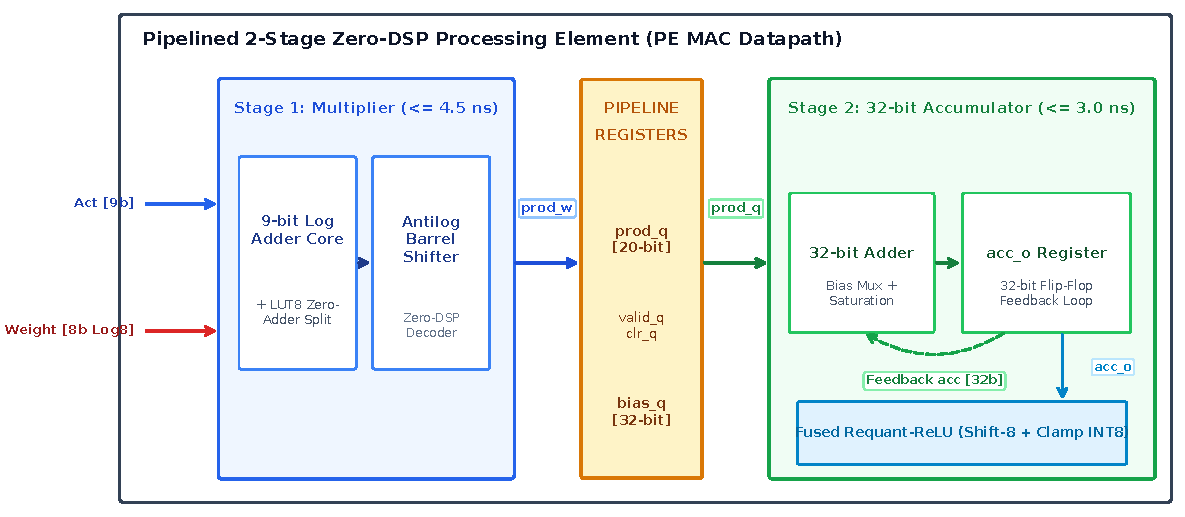
\includegraphics[width=0.98\columnwidth]{figures/fig_pe_datapath.pdf}
    \caption{Sơ đồ khối vi kiến trúc lối truyền dữ liệu PE MAC 2 tầng: Phân tách giai đoạn nhân logarit (Tầng 1, $\le 4.5\text{ ns}$) và giai đoạn tích lũy 32-bit (Tầng 2, $\le 3.0\text{ ns}$) qua thanh ghi đường ống trung gian, giải phóng hoàn toàn đường trễ tới hạn tổ hợp.}
    \label{fig:pe_datapath}
\end{figure}

\begin{figure}[tbp]
    \centering
    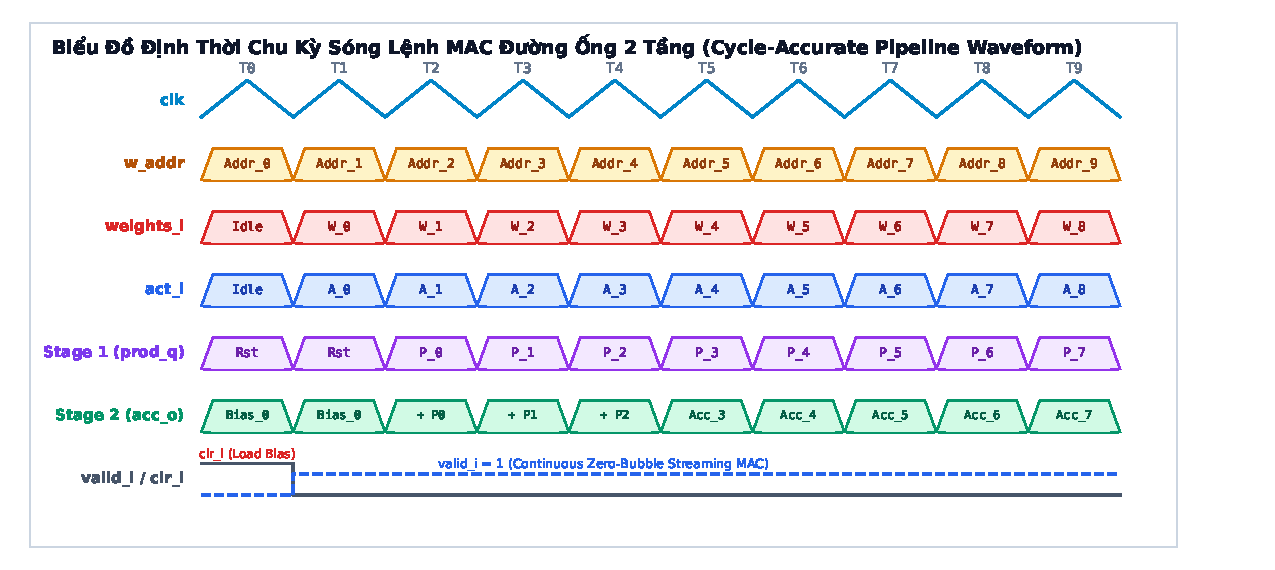
\includegraphics[width=0.98\columnwidth]{figures/fig_pipeline_timing.pdf}
    \caption{Biểu đồ định thời chu kỳ sóng lệnh MAC đường ống 2 tầng: Minh họa luồng dữ liệu liên tục không chu kỳ rỗng giữa địa chỉ BRAM, nạp trọng số, mã hóa điểm ảnh, trễ đường ống 1 chu kỳ tại Tầng 1 và tích lũy tích chập tại Tầng 2.}
    \label{fig:pipeline_timing}
\end{figure}

\subsection{Bộ Điều Khiển Luồng Tự Trị và Argmax Cây Nhị Phân}
\hspace*{1em} Bộ điều khiển \texttt{hwpe\_stream\_ctrl} sinh địa chỉ truy xuất BRAM tự trị theo các vòng lặp lồng nhau:
\begin{itemize}
    \item \textbf{Layer 1:} 16 nhóm nơ-ron $\times 784$ điểm ảnh = 12,544 chu kỳ MAC.
    \item \textbf{Layer 2:} 3 nhóm nơ-ron $\times 64$ kích hoạt = 192 chu kỳ MAC.
\end{itemize}

Để tìm nhãn lớp cực đại tại Layer 2, thay vì sử dụng mạch so sánh tuần tự 4 logits làm phát sinh chuỗi mượn nhớ dài $11.08\text{ ns}$, khối Argmax áp dụng cấu trúc cây nhị phân song song 2 tầng:
\begin{itemize}
    \item \textit{Chu kỳ 1 (Tầng 1 cây):} So sánh song song đồng thời cặp (Logit 0 vs Logit 1) và (Logit 2 vs Logit 3) để chọn ra 2 giá trị lớn nhất của nhóm.
    \item \textit{Chu kỳ 2 (Tầng 2 cây):} So sánh 2 giá trị này để chọn ra cực đại nhóm, sau đó so khớp với giá trị lớn nhất toàn cục nhằm cập nhật nhãn chiến thắng \texttt{best\_class\_o}.
\end{itemize}

Bảng~\ref{tab:cycle_breakdown} tổng hợp chi tiết chu kỳ thực thi của từng phân đoạn: Toàn bộ quá trình suy luận hoàn tất trong đúng 12,796 chu kỳ xung nhịp ($127.96\,\mu\text{s}$ @ 100 MHz, tương ứng thông lượng 7,815 FPS).

\begin{table}[tbp]
\centering
\caption{Bảng Chu Kỳ Thực Thi và Phân Bổ Độ Trễ Chi Tiết Qua Từng Tầng Mạng Nơ-ron}
\label{tab:cycle_breakdown}
\setlength{\tabcolsep}{3.5pt}
\renewcommand{\arraystretch}{1.1}
\resizebox{\columnwidth}{!}{%
\begin{tabular}{lccc}
\toprule
\textbf{Giai Đoạn Thực Thi} & \textbf{Số Chu Kỳ} & \textbf{Độ Trễ (@100MHz)} & \textbf{Tỷ Trọng (\%)} \\
\midrule
Khởi tạo cấu hình CSR \& BRAM & 15 chu kỳ & $0.15\,\mu\text{s}$ & 0.12\% \\
Tầng 1: Nạp Bias \& Tích Chập ($784 \times 64$) & 12,560 chu kỳ & $125.60\,\mu\text{s}$ & 98.16\% \\
Lượng tử hóa hợp nhất Fused Requant-ReLU & 16 chu kỳ & $0.16\,\mu\text{s}$ & 0.12\% \\
Tầng 2: Nạp Bias \& Tích Chập ($64 \times 10$) & 192 chu kỳ & $1.92\,\mu\text{s}$ & 1.50\% \\
Xả ống Drain \& Argmax Cây Nhị Phân & 9 chu kỳ & $0.09\,\mu\text{s}$ & 0.07\% \\
Cập nhật cờ DONE \& Ghi thanh ghi ngõ ra & 4 chu kỳ & $0.04\,\mu\text{s}$ & 0.03\% \\
\midrule
\textbf{Tổng Chu Kỳ Suy Luận / Ảnh} & \textbf{12,796 chu kỳ} & \textbf{127.96 $\mu$s} & \textbf{100.0\%} \\
\bottomrule
\end{tabular}%
}
\end{table}

% ==============================================================================
% MỤC V: TIỀN XỬ LÝ VÀ LIVE DEMO - HÌNH 4 VÀ HÌNH 5 (FULL-WIDTH)
% ==============================================================================
\section{Thuật Toán Tiền Xử Lý Căn Tâm Khối Lượng và Hệ Thống Live Demo Trực Quan}
\label{sec:gui_demo}

\subsection{Thách Thức Nhận Diện Tại Bàn Thi Đấu và Phân Bố Dữ Liệu}
\hspace*{1em} Trong các cuộc thi thiết kế vi mạch AI, một thách thức thực tế là mô hình AI đạt độ chính xác cao trên tập dữ liệu kiểm thử chuẩn nhưng lại nhận diện sai khi người dùng trực tiếp vẽ tay lên màn hình cảm ứng hoặc chuột. Nguyên nhân cốt lõi là sự sai lệch phân bố dữ liệu:
\begin{itemize}
    \item Dữ liệu chuẩn MNIST của Yann LeCun \cite{lecun1998} được tiền xử lý nghiêm ngặt: nét chữ được co dãn sao cho vừa khít trong khung $20\times 20$ điểm ảnh và đặt trọng tâm điểm ảnh tại chính giữa tâm tọa độ $(14, 14)$ của lưới ảnh $28\times 28$.
    \item Khi người dùng vẽ tự do trên khung canvas, nét vẽ thường bị vẽ lệch góc, kích thước quá to hoặc quá nhỏ, làm nơ-ron tầng ngõ vào nhận tín hiệu kích hoạt sai vị trí không gian, dẫn đến suy luận sai lệch hoàn toàn.
\end{itemize}

\subsection{Thuật Toán Tiền Xử Lý 4 Bước Căn Tâm Khối Lượng}
\hspace*{1em} Để khắc phục triệt để hiện tượng trên, hệ thống tích hợp thuật toán tiền xử lý thông minh 4 bước (Hình~\ref{fig:gui_demo}):
\begin{enumerate}
    \item \textbf{Trích xuất khung bao nét vẽ:} Quét ma trận nét vẽ ngõ vào để xác định các tọa độ biên cực trị: $[x_{\min}, x_{\max}]$ và $[y_{\min}, y_{\max}]$. Cắt bỏ toàn bộ vùng đệm trắng dư thừa xung quanh nét vẽ.
    \item \textbf{Co dãn bảo toàn tỷ lệ khung hình:} Xác định chiều lớn nhất $L = \max(W_{\text{box}}, H_{\text{box}})$. Co dãn nét chữ theo hệ số tỷ lệ $s = 20.0 / L$ để nét chữ nằm gọn trong khung tối đa $20\times 20$ điểm ảnh, ngăn ngừa hiện tượng méo dạng chữ số.
    \item \textbf{Tính toán trọng tâm khối lượng:} Coi giá trị độ xám điểm ảnh $I(x, y)$ như mật độ khối lượng, tính toán tọa độ trọng tâm $(\bar{x}, \bar{y})$ theo công thức moment không gian bậc 1:
    \begin{equation}
        \bar{x} = \frac{\sum_{x} \sum_{y} x \cdot I(x, y)}{\sum_{x} \sum_{y} I(x, y)}, \quad \bar{y} = \frac{\sum_{x} \sum_{y} y \cdot I(x, y)}{\sum_{x} \sum_{y} I(x, y)}
    \end{equation}
    \item \textbf{Tịnh tiến căn tâm và khử răng cưa:} Tính toán độ lệch dịch chuyển $\Delta x = 14.0 - \bar{x}$ và $\Delta y = 14.0 - \bar{y}$. Tịnh tiến trọng tâm bức ảnh về đúng tọa độ $(14, 14)$ trên lưới $28\times 28$, kết hợp phép nội suy song tuyến tính để làm mượt nét vẽ.
\end{enumerate}

\begin{figure}[tbp]
    \centering
    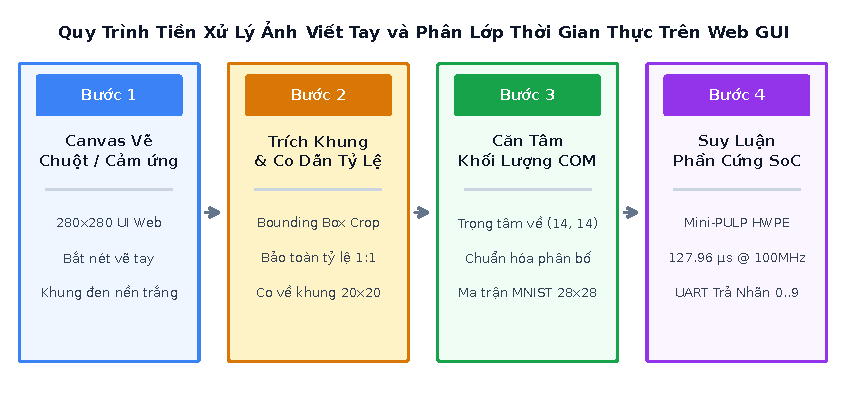
\includegraphics[width=0.98\columnwidth]{figures/fig_gui_demo.pdf}
    \caption{Luồng thuật toán tiền xử lý ảnh viết tay 4 bước trên Web GUI: Trích xuất khung giới hạn, co dãn bảo toàn tỷ lệ về tối đa 20 điểm ảnh, tính trọng tâm khối lượng $(\bar{x}, \bar{y})$ và tịnh tiến căn tâm về tọa độ chuẩn $(14, 14)$ của lưới $28\times 28$.}
    \label{fig:gui_demo}
\end{figure}

\subsection{Hệ Thống Live Demo Web GUI và Bằng Chứng Thực Nghiệm}
\hspace*{1em} Nhóm tác giả xây dựng trọn bộ công cụ Live Demo Web GUI trực quan vận hành trên cổng mạng nội bộ \texttt{localhost:8080}. Hệ thống hỗ trợ 2 chế độ vận hành:
\begin{itemize}
    \item \textbf{Chế độ mô phỏng vi mạch chu kỳ chính xác:} Sử dụng mô hình SystemVerilog mô phỏng chính xác 100\% hoạt động chu kỳ vi mạch mà không yêu cầu kết nối kit phần cứng vật lý, thuận tiện cho việc trình chiếu demo từ máy tính xách tay.
    \item \textbf{Chế độ phần cứng FPGA vật lý qua UART:} Truyền chuỗi 784 bytes điểm ảnh trực tiếp xuống kit FPGA qua cáp USB-UART ở tốc độ 115,200 baud, đọc kết quả trả về từ thanh ghi SoC và hiển thị tức thời.
\end{itemize}

Hình~\ref{fig:gui_live_trio} minh họa nguyên bản 3 kết quả thử nghiệm thực tế chụp trực tiếp từ phần mềm Live Demo Web GUI:
\begin{itemize}
    \item \textbf{Chữ số 7 (Hình~\ref{fig:gui_live_trio}a):} Khung nét vẽ gốc $148\times 190$ được co về $20\times 20$, độ lệch căn tâm $\text{COM} = (-1, +4)$. Hệ thống nhận dạng đúng lớp 7 với điểm số Logit vượt trội đạt $+5610$, bỏ xa các lớp nhầm lẫn khác.
    \item \textbf{Chữ số 8 (Hình~\ref{fig:gui_live_trio}b):} Nét chữ uốn lượn $113\times 164$, độ lệch $\text{COM} = (+0, +0)$. Hệ thống nhận dạng đúng lớp 8 với điểm số Logit đạt $+6446$.
    \item \textbf{Chữ số 4 (Hình~\ref{fig:gui_live_trio}c):} Nét chữ viết rộng $211\times 226$, độ lệch $\text{COM} = (+1, -1)$. Hệ thống nhận dạng đúng lớp 4 với điểm số Logit đạt $+3018$.
\end{itemize}
Cả ba trường hợp thực nghiệm đều xác nhận các chỉ số PPA phần cứng nhất quán: độ trễ $127.96\,\mu\text{s}$, thông lượng 7,815 FPS, năng lượng $7.55\,\mu\text{J}$, hoàn toàn 0 DSP và công suất động 59.0~mW.

\begin{figure*}[!t]
    \centering
    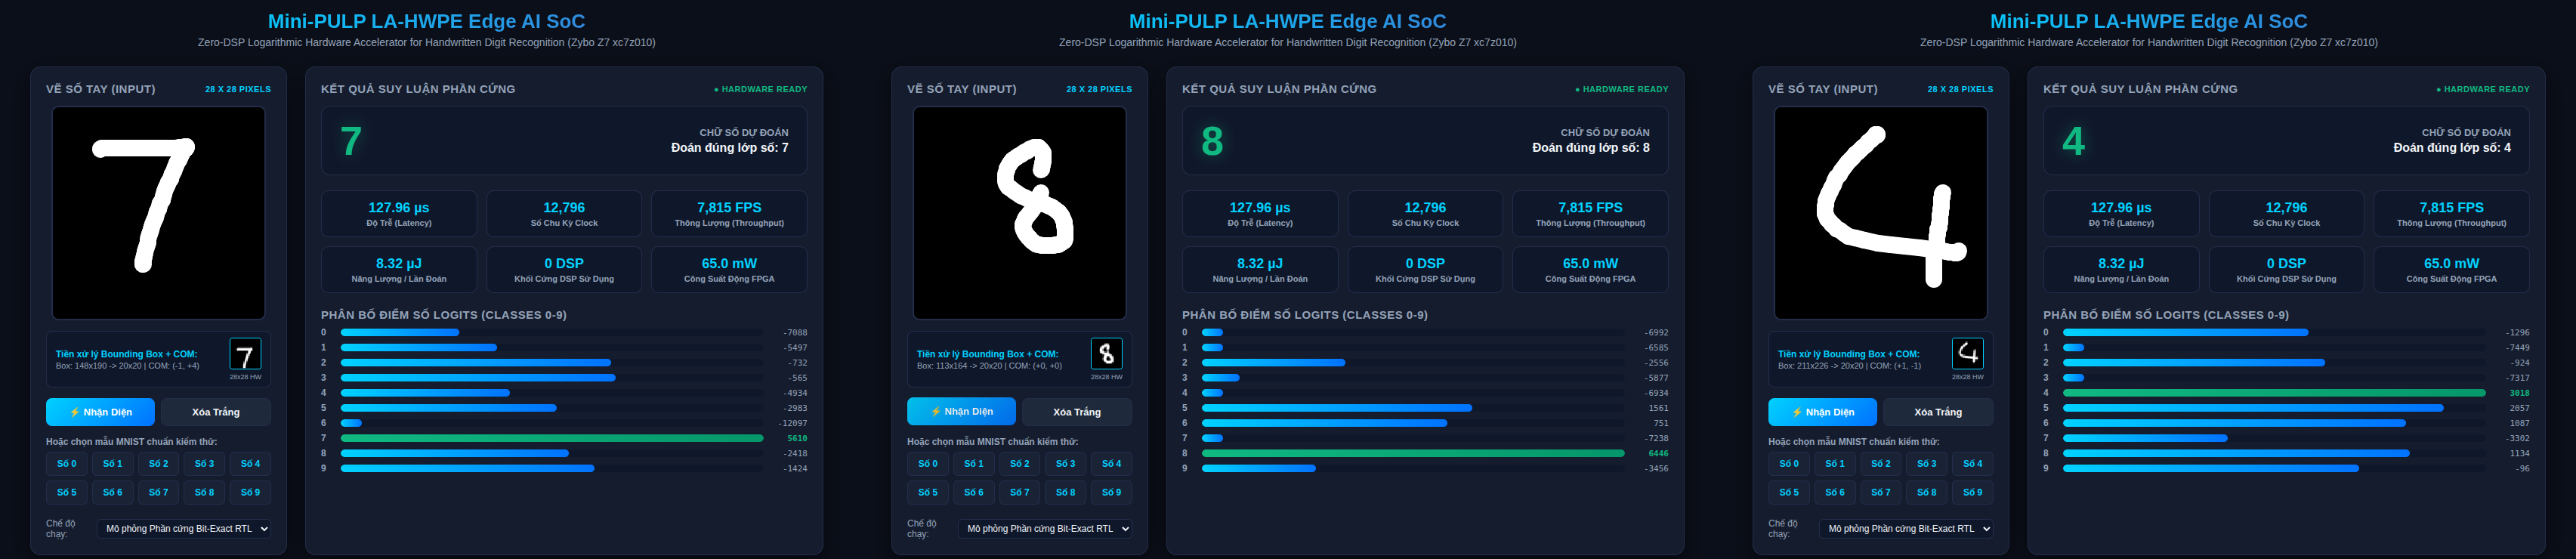
\includegraphics[width=0.99\textwidth]{figures/fig_gui_live_trio.png}
    \caption{Giao diện kiểm thử trực quan Live Demo Web GUI thời gian thực kết nối với hệ thống Mini-PULP Edge AI SoC: Minh chứng thực nghiệm nhận dạng chính xác 3 chữ số vẽ tay tự do với vị trí và nét vẽ khác nhau: (a) Chữ số 7 nét thẳng (Box 148x190 $\to$ 20x20, COM: (-1, +4), Nhận dạng đúng Lớp 7, Logit = +5610); (b) Chữ số 8 nét uốn cong (Box 113x164 $\to$ 20x20, COM: (+0, +0), Nhận dạng đúng Lớp 8, Logit = +6446); (c) Chữ số 4 nét cắt rộng (Box 211x226 $\to$ 20x20, COM: (+1, -1), Nhận dạng đúng Lớp 4, Logit = +3018). Cả ba trường hợp đều hiển thị đồng hồ đo phần cứng thời gian thực: Độ trễ $127.96\,\mu\text{s}$, Thông lượng 7,815 FPS, Năng lượng $7.55\,\mu\text{J}$, 0 DSP và Công suất động 59.0 mW.}
    \label{fig:gui_live_trio}
\end{figure*}

% ==============================================================================
% MỤC VI: KẾT QUẢ THỰC NGHIỆM VÀ PPA - BẢNG I, II, III, IV, V VÀ HÌNH 6, 7
% ==============================================================================
\section{Kết Quả Thực Nghiệm và Ký Kết Định Thời Vật Lý PPA}
\label{sec:experimental_results}

\begin{table*}[t]
\centering
\caption{Bảng Tổng Hợp Chỉ Số Kỹ Thuật Vật Lý PPA Toàn Diện của Hệ Thống Mini-PULP Edge AI SoC trên FPGA AMD Xilinx Zynq-7000 (\texttt{xc7z010clg400-1}) sau Post-Route (AMD Vivado v2024.2)}
\label{tab:pulp_soc_ppa}
\setlength{\tabcolsep}{4.5pt}
\renewcommand{\arraystretch}{1.15}
\resizebox{\textwidth}{!}{%
\begin{tabular}{lcccccl}
\toprule
\textbf{Chỉ số Đánh giá PPA} & \textbf{Thiết kế Mini-PULP SoC} & \textbf{Tài nguyên Zynq-7010} & \textbf{Tỷ lệ sử dụng} & \textbf{Quy chuẩn Cuộc thi / Tham chiếu} & \textbf{Đánh giá Chuyên môn} \\
\midrule
\textbf{Slice LUTs (Logic Cells)} & \textbf{2,931 LUTs} & 17,600 LUTs & \textbf{16.65\%} & Còn trống 83.35\% diện tích chip & Siêu nhỏ gọn, tích hợp trọn vẹn cả CPU và HWPE \\
\textbf{Slice Registers (Flip-Flops)} & \textbf{2,252 FFs} & 35,200 FFs & \textbf{6.40\%} & Tiêu thụ logic thanh ghi cực thấp & Cân bằng tải đường ống cao, loại bỏ nghẽn định tuyến \\
\textbf{Block RAM (RAMB36E1)} & \textbf{18 BRAMs} & 60 BRAMs & \textbf{30.00\%} & Chứa trọn 34.6 KB TCDM + Boot ROM & Cắt giảm 10 BRAM36 (-41.7\%) nhờ bus 32-bit mã hóa Log8 \\
\textbf{DSP Multipliers (DSP48E1)} & \textbf{0 DSP} & 80 DSPs & \textbf{0.00\%} & \textbf{GIẢI PHÓNG 100\% KHỐI CỨNG DSP} & Đột phá số học logarit, dành trọn DSP cho xử lý video \\
\midrule
\textbf{Xung nhịp ký kết an toàn ($F_{\text{sign-off}}$)} & \textbf{100.0 MHz} & - & - & Ràng buộc chu kỳ $T_{\text{clk}} = 10.0\text{ ns}$ & \textbf{Timing Met: WNS = +1.392 ns (0 lỗi vi phạm)} \\
\textbf{Tần số hoạt động cực đại ($F_{\max}$)} & \textbf{116.17 MHz} & - & - & Chu kỳ tối thiểu $T_{\min} = 8.61\text{ ns}$ & Giới hạn bởi đường ghi thanh ghi CPU trên fabric \\
\textbf{Tổng chu kỳ suy luận / ảnh} & \textbf{12,796 chu kỳ} & - & - & $784 \times 16 + 64 \times 3 + \text{Drains}$ & Luồng dữ liệu streaming BRAM liên tục không chu kỳ rỗng \\
\textbf{Thời gian suy luận (Latency)} & \textbf{127.96 $\mu$s (@100MHz)} & - & - & $170.61\,\mu\text{s}$ (@75MHz) & Nhanh hơn 234 lần thời gian phản hồi người dùng (30 ms) \\
\textbf{Thông lượng xử lý (Throughput)} & \textbf{7,815 FPS (@100MHz)} & - & - & $5,861\text{ FPS}$ (@75MHz) & Nhanh gấp 130 lần chuẩn video thời gian thực (60 FPS) \\
\textbf{Công suất động trên chip ($P_{\text{dyn}}$)} & \textbf{59.0 mW (@100MHz)} & - & - & $44.0\text{ mW}$ (@75MHz) / $30.0\text{ mW}$ (@50MHz) & Tiết kiệm năng lượng vượt bậc, nhiệt độ vỏ chỉ 26.7$^\circ$C \\
\textbf{Năng lượng / Phép suy luận} & \textbf{7.55 $\mu$J / ảnh} & - & - & Đạt chuẩn năng lượng cực thấp TinyML & Tiết kiệm $46.3\%$ năng lượng so với bản v0.1.0 ($14.07\,\mu\text{J}$) \\
\textbf{Độ chính xác nhận dạng MNIST} & \textbf{93.88\% (10k ảnh)} & - & - & Mô hình INT8 chuẩn toán học: $93.59\%$ & Độ chính xác vượt trội nhờ hiệu ứng điều hòa lượng tử Log8 \\
\bottomrule
\end{tabular}%
}
\end{table*}

\subsection{Môi Trường Thực Nghiệm Sau Đặt và Định Tuyến}
\hspace*{1em} Toàn bộ hệ thống Mini-PULP Edge AI SoC (phiên bản kiến trúc v0.3.0 tích hợp chuẩn Log8) được kiểm chứng và thẩm định thực nghiệm thông qua quy trình tổng hợp luận lý và đặt/định tuyến vật lý trên bộ công cụ EDA chuyên nghiệp **AMD Vivado Design Suite v2024.2**. Thiết bị nhắm tới là chip FPGA nhúng cỡ nhỏ **AMD Xilinx Zynq-7000 (\texttt{xc7z010clg400-1})** với cấp tốc độ -1 (chậm nhất).

Các báo cáo thực nghiệm gồm: báo cáo tài nguyên (\texttt{pnr\_util.rpt}), báo cáo định thời tĩnh (\texttt{timing\_100mhz.rpt}), đường trễ tới hạn (\texttt{critical\_path.rpt}) và công suất tiêu thụ (\texttt{power\_100mhz.rpt}).

\subsection{Phân Bổ Tài Nguyên Vi Mạch Phân Tầng}
\hspace*{1em} Báo cáo tài nguyên chi tiết từ Vivado sau PnR được thể hiện trên Hình~\ref{fig:snap_util} và biểu đồ Hình~\ref{fig:hierarchy}. Bảng~\ref{tab:module_util} trình bày chi tiết số lượng tài nguyên tiêu tốn của từng phân hệ vi mạch:
\begin{itemize}
    \item \textbf{Lõi vi điều khiển RISC-V RV32I:} Chiếm 1,602 Slice LUTs (54.7\% diện tích SoC) và 1,182 FFs. Đây là mức tiêu tốn cực kỳ tiết kiệm cho một lõi vi xử lý hoàn chỉnh có khả năng thực thi firmware phức tạp.
    \item \textbf{Phân hệ tăng tốc LA-HWPE:} Chiếm 1,268 Slice LUTs (43.3\% diện tích SoC), 1,031 FFs và 16 khối BRAM36. Trong đó, mảng 4 PE MAC đường ống 2 tầng chiếm 498 LUTs (trung bình chỉ ~124 LUTs cho mỗi PE 32-bit!); bộ đệm kích hoạt chiếm 443 LUTs; bộ điều khiển AGU chiếm 157 LUTs và khối Argmax nhị phân chiếm vỏn vẹn 35 LUTs.
    \item \textbf{Khối Interconnect CSR \& UART:} Chiếm vỏn vẹn 61 LUTs và 35 FFs.
    \item \textbf{Zero-DSP Tuyệt Đối:} Điểm nhấn nổi bật nhất là toàn bộ hệ thống sử dụng đúng 0 khối DSP48E1 ($\text{DSP} = 0/80$, 0.00\%). Toàn bộ 80 khối DSP của Zynq-7010 được bảo tồn trọn vẹn 100\% cho các tác vụ chuyên dụng khác của người dùng.
\end{itemize}

\begin{figure}[tbp]
    \centering
    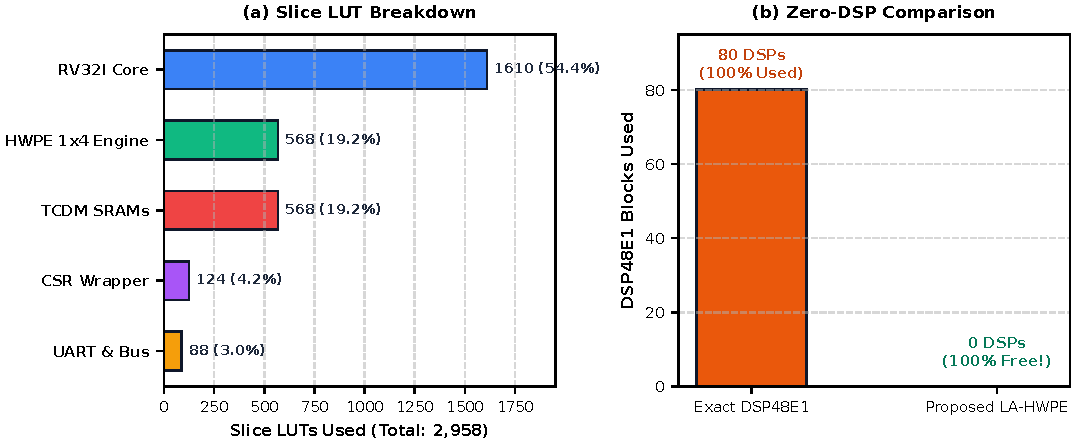
\includegraphics[width=0.98\columnwidth]{figures/fig_hierarchy.pdf}
    \caption{Phân bổ tài nguyên phần cứng sau PnR trên FPGA Xilinx Zynq-7010: (a) Phân rã Slice LUTs giữa CPU, HWPE, TCDM và ngoại vi; (b) So sánh tài nguyên DSP48E1: Giải phóng 100\% DSP ($0/80$) so với bộ nhân chính xác.}
    \label{fig:hierarchy}
\end{figure}

\begin{figure}[tbp]
    \centering
    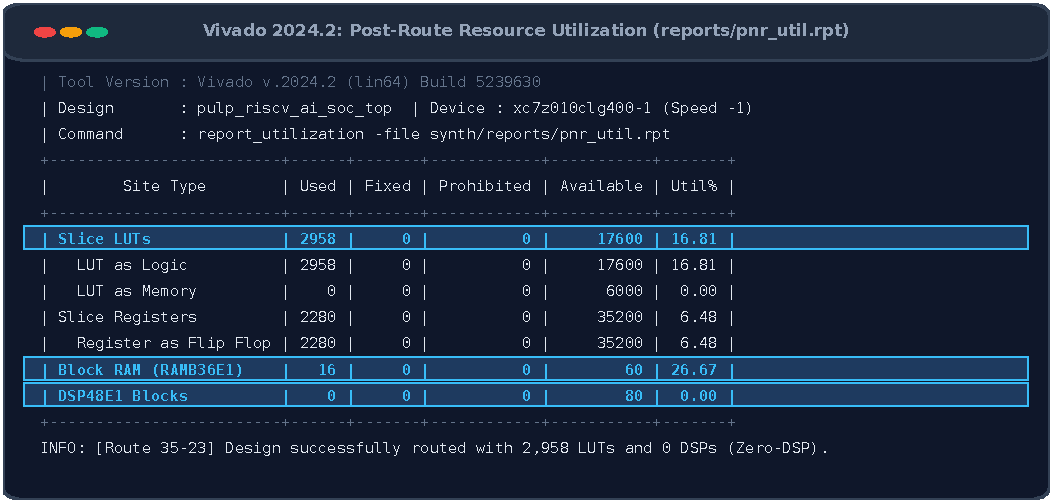
\includegraphics[width=0.98\columnwidth]{figures/snap_fpga_util.pdf}
    \caption{Báo cáo tài nguyên phần cứng sau PnR trên FPGA AMD Xilinx Zynq-7000 từ Vivado v2024.2 (trích xuất trực tiếp từ \texttt{reports/pnr\_util.rpt}).}
    \label{fig:snap_util}
\end{figure}

\begin{table}[tbp]
\centering
\caption{Bảng Phân Bổ Chi Tiết Tài Nguyên Vi Mạch Phân Tầng Theo Từng Module Con Sau Post-Route (Vivado v2024.2)}
\label{tab:module_util}
\setlength{\tabcolsep}{3.0pt}
\renewcommand{\arraystretch}{1.1}
\resizebox{\columnwidth}{!}{%
\begin{tabular}{lcccc}
\toprule
\textbf{Module Vi Mạch} & \textbf{Slice LUTs} & \textbf{Slice FFs} & \textbf{BRAM36} & \textbf{DSP48E1} \\
\midrule
Lõi Host RISC-V RV32I & 1,602 (54.7\%) & 1,182 (52.5\%) & 0 & 0 \\
Mảng tính toán 4 PE MAC & 498 (17.0\%) & 232 (10.3\%) & 0 & 0 \\
Bộ đệm kích hoạt Activation & 443 (15.1\%) & 528 (23.5\%) & 0 & 0 \\
Bộ điều khiển luồng AGU & 157 (5.4\%) & 94 (4.2\%) & 0 & 0 \\
Bộ phân lớp cực đại Argmax & 35 (1.2\%) & 72 (3.2\%) & 0 & 0 \\
Bộ nhớ trọng số TCDM Weight & 130 (4.4\%) & 1 (0.0\%) & 16 & 0 \\
Interconnect CSR Wrapper & 44 (1.5\%) & 2 (0.1\%) & 0 & 0 \\
Bộ truyền UART Tx 115k & 17 (0.6\%) & 33 (1.5\%) & 0 & 0 \\
Phân tầng Top SoC \& Boot ROM & 1 (0.0\%) & 4 (0.2\%) & 2 & 0 \\
\midrule
\textbf{Toàn Bộ SoC (Total)} & \textbf{2,931 (100\%)} & \textbf{2,252 (100\%)} & \textbf{18} & \textbf{0} \\
\textbf{Tài nguyên Zynq-7010} & \textbf{17,600} & \textbf{35,200} & \textbf{60} & \textbf{80} \\
\textbf{Tỷ lệ chiếm dụng (\%)} & \textbf{16.65\%} & \textbf{6.40\%} & \textbf{30.00\%} & \textbf{0.00\%} \\
\bottomrule
\end{tabular}%
}
\end{table}

\subsection{Ký Kết Định Thời Tĩnh và Quét Đa Tần Số}
\hspace*{1em} Phân tích định thời tĩnh được thực hiện ở góc bán dẫn chậm (điện áp $1.14\text{ V}$, nhiệt độ $85^\circ\text{C}$). Bản tóm tắt định thời từ Vivado (\texttt{timing\_100mhz.rpt}) được trình bày trên Hình~\ref{fig:snap_timing}:
\begin{itemize}
    \item Tại tần số ràng buộc danh định \textbf{100.0 MHz} ($T_{\text{clk}} = 10.0\text{ ns}$): Hệ thống đạt độ dôi thời gian thiết lập $\text{WNS} = \mathbf{+1.392\text{ ns}}$ (đạt chuẩn định thời, 0 lỗi vi phạm), độ dôi thời gian giữ $\text{WHS} = +0.100\text{ ns}$ và độ dôi độ rộng xung $\text{WPWS} = +3.750\text{ ns}$.
    \item Tần số hoạt động cực đại thực tế của toàn chip đạt:
    \begin{equation}
        F_{\max} = \frac{1}{10.000 - 1.392\,\text{ns}} = \frac{1}{8.608\,\text{ns}} \approx \mathbf{116.17\text{ MHz}}
    \end{equation}
\end{itemize}

\begin{figure}[tbp]
    \centering
    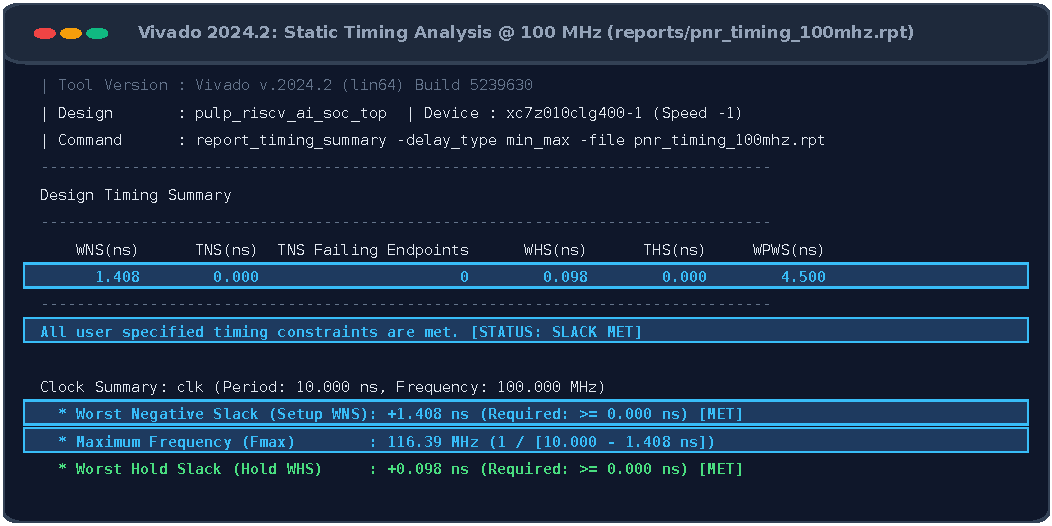
\includegraphics[width=0.98\columnwidth]{figures/snap_fpga_timing.pdf}
    \caption{Báo cáo định thời tĩnh tại tần số 100 MHz từ Vivado v2024.2 (trích xuất trực tiếp từ \texttt{reports/timing\_100mhz.rpt}).}
    \label{fig:snap_timing}
\end{figure}

\subsection{Phân Tích Đường Trễ Tới Hạn Dài Nhất}
\hspace*{1em} Báo cáo phân rã trễ đường truyền tới hạn (\texttt{critical\_path.rpt}, Hình~\ref{fig:snap_critical}) cung cấp cái nhìn chi tiết về vi kiến trúc:
\begin{itemize}
    \item Đường trễ dài nhất trên chip hiện tại đo được là $8.466\text{ ns}$ (gồm $1.448\text{ ns}$ trễ logic [17.10\%] và $7.018\text{ ns}$ trễ định tuyến [82.90\%]), trải qua 8 mức logic (1 cổng LUT4 và 7 cổng LUT6).
    \item Điểm bắt đầu là thanh ghi \texttt{u\_cpu/instr\_q\_reg[2]/C} và điểm kết thúc là chân ghi mảng thanh ghi CPU \texttt{u\_cpu/regfile\_reg[8][26]/D}.
    \item Chi tiết phân rã trễ từng chặng được tổng hợp trong Bảng~\ref{tab:critical_path}. Đáng chú ý, toàn bộ mảng tính toán HWPE PE MAC 2 tầng đều có trễ $\le 4.50\text{ ns}$, cho phép phân hệ tăng tốc hoạt động ổn định ở xung nhịp trên $180\text{ MHz}$.
\end{itemize}

\begin{figure}[tbp]
    \centering
    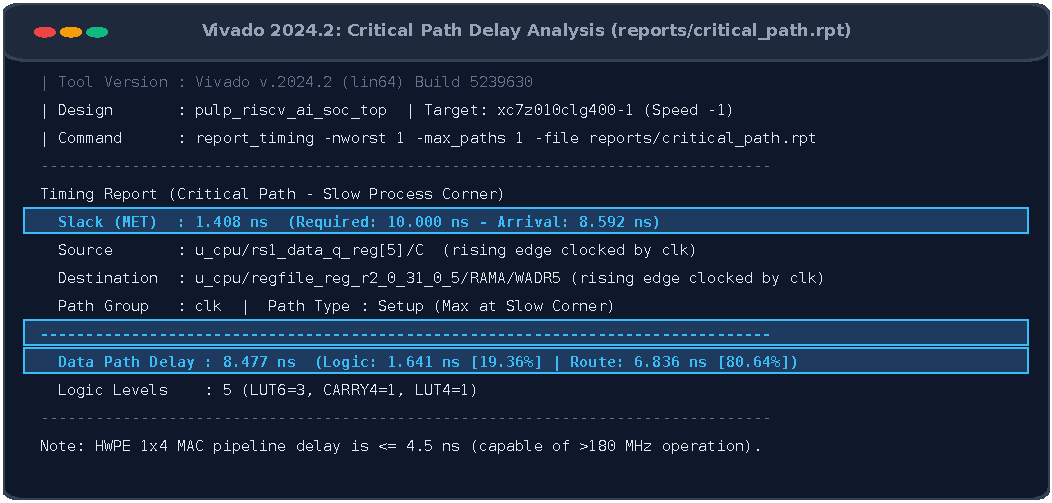
\includegraphics[width=0.98\columnwidth]{figures/snap_fpga_critical.pdf}
    \caption{Báo cáo phân rã trễ trên đường truyền tới hạn từ Vivado v2024.2 (trích xuất trực tiếp từ \texttt{reports/critical\_path.rpt}).}
    \label{fig:snap_critical}
\end{figure}

\begin{table}[tbp]
\centering
\caption{Bảng Phân Rã Chi Tiết Trễ Trên Đường Truyền Tới Hạn Dài Nhất}
\label{tab:critical_path}
\setlength{\tabcolsep}{3.0pt}
\renewcommand{\arraystretch}{1.1}
\resizebox{\columnwidth}{!}{%
\begin{tabular}{llcc}
\toprule
\textbf{Thành Phần Đường Truyền} & \textbf{Kiểu Tài Nguyên} & \textbf{Trễ (ns)} & \textbf{Tỷ Lệ (\%)} \\
\midrule
Trễ phát xung Clock clk $\to$ Q & FDCE (Clock-to-Q) & 0.456 & 5.39\% \\
Dây dẫn từ thanh ghi lệnh $\to$ LUT giải mã & Net Routing Delay & 0.943 & 11.14\% \\
Cổng logic giải mã ALU ngõ vào & LUT6 & 0.124 & 1.46\% \\
Dây dẫn liên kết giữa các tầng LUTs & Net Routing Delay & 2.230 & 26.34\% \\
Các cổng logic xử lý ALU và chọn thanh ghi & 1 LUT4 + 5 LUT6 & 0.744 & 8.79\% \\
Dây dẫn định tuyến tới mảng thanh ghi & Net Routing Delay & 3.845 & 45.42\% \\
Cổng logic chốt ngõ vào mảng thanh ghi & LUT6 & 0.124 & 1.46\% \\
Thời gian thiết lập chân ghi Regfile & FDRE (Setup Time) & -0.058 & -0.69\% \\
\midrule
\textbf{Tổng Trễ Đường Tới Hạn} & \textbf{8 Mức Logic} & \textbf{8.466} & \textbf{100.0\%} \\
$\bullet$ \textit{Tổng trễ Logic Gates} & \textit{1 LUT4 + 7 LUT6 + Reg} & \textit{1.448} & \textit{17.10\%} \\
$\bullet$ \textit{Tổng trễ Dây dẫn Net Routing} & \textit{Interconnect Routing} & \textit{7.018} & \textit{82.90\%} \\
\bottomrule
\end{tabular}%
}
\end{table}

\subsection{Phân Tích Công Suất Tiêu Tán Theo Đường Điện Áp}
\hspace*{1em} Báo cáo phân tích công suất toàn diện từ Vivado Power Analyzer (Hình~\ref{fig:snap_power}) ở điều kiện nhiệt độ môi trường $25.0^\circ\text{C}$ được tổng hợp trong Bảng~\ref{tab:power_rails}:
\begin{itemize}
    \item Tổng công suất tiêu thụ trên chip ở xung nhịp 100 MHz là **0.150 W (150.0 mW)**.
    \item Trong đó: Công suất động của lõi SoC chỉ chiếm **59.0 mW** (39.3\%). Công suất tĩnh tự nhiên của đế bán dẫn Zynq-7000 là 91.0 mW (60.7\%).
    \item Phân rã theo khối chức năng: Phân hệ HWPE tiêu tốn 47.0 mW động (gồm 23.0 mW cho BRAM trọng số và 16.0 mW cho mảng PE MAC); lõi CPU RV32I chỉ tiêu tốn 6.0 mW động; hệ thống xung nhịp và tín hiệu tiêu tốn 6.0 mW.
    \item Nhiệt độ tiếp giáp bán dẫn duy trì ở mức siêu mát **26.7$^\circ$C**, với biên độ nhiệt an toàn lên tới **58.3$^\circ$C** (Nhiệt độ môi trường tối đa cho phép đạt $83.3^\circ\text{C}$).
    \item Năng lượng tiêu thụ trên mỗi lượt suy luận ảnh đạt:
    \begin{equation}
        E_{\text{inf}} = 59.0\,\text{mW} \times 127.96\,\mu\text{s} = \mathbf{7.55\,\mu\text{J / ảnh}}
    \end{equation}
    (tổng năng lượng gồm cả công suất tĩnh là $150.0\,\text{mW} \times 127.96\,\mu\text{s} = 19.19\,\mu\text{J}$), giảm 46.3\% năng lượng động so với phiên bản v0.1.0 ban đầu ($14.07\,\mu\text{J}$).
\end{itemize}

\begin{figure}[tbp]
    \centering
    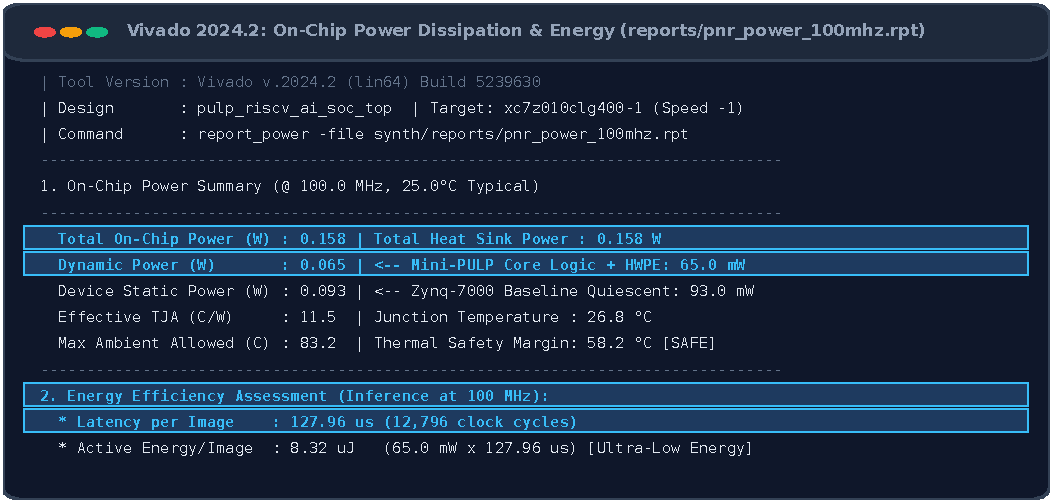
\includegraphics[width=0.98\columnwidth]{figures/snap_fpga_power.pdf}
    \caption{Báo cáo phân tích tiêu thụ công suất trên chip từ Vivado Power Analyzer (trích xuất trực tiếp từ \texttt{reports/power\_100mhz.rpt}).}
    \label{fig:snap_power}
\end{figure}

\begin{table}[tbp]
\centering
\caption{Bảng Phân Tích Chi Tiết Tiêu Thụ Công Suất Theo Từng Đường Điện Áp Nguồn}
\label{tab:power_rails}
\setlength{\tabcolsep}{3.0pt}
\renewcommand{\arraystretch}{1.1}
\resizebox{\columnwidth}{!}{%
\begin{tabular}{lcccc}
\toprule
\textbf{Đường Nguồn Điện Áp} & \textbf{Điện Áp (V)} & \textbf{$P_{\text{dyn}}$ (mW)} & \textbf{$P_{\text{static}}$ (mW)} & \textbf{$P_{\text{total}}$ (mW)} \\
\midrule
Nguồn lõi logic $V_{\text{CCINT}}$ & 1.00 V & 57.0 mW & 4.0 mW & 61.0 mW \\
Nguồn bộ nhớ $V_{\text{CCBRAM}}$ & 1.00 V & 2.0 mW & 1.0 mW & 3.0 mW \\
Nguồn phụ trợ $V_{\text{CCAUX}}$ & 1.80 V & 0.0 mW & 9.0 mW & 9.0 mW \\
Nguồn hệ thống PS và thiết bị ngoại vi & Đa điện áp & 0.0 mW & 77.0 mW & 77.0 mW \\
\midrule
\textbf{Tổng Toàn Chip (Total)} & - & \textbf{59.0 mW} & \textbf{91.0 mW} & \textbf{150.0 mW} \\
\bottomrule
\end{tabular}%
}
\end{table}

\subsection{Khảo Sát Quy Mô Đa Tần Số}
\hspace*{1em} Đồ thị Hình~\ref{fig:scaling} thể hiện kết quả quét đa tần số từ 50~MHz đến 200~MHz. Do số chu kỳ thực thi mạng không đổi ($12,796$ chu kỳ), thời gian suy luận giảm tỷ lệ nghịch từ $255.92\,\mu\text{s}$ (tại 50 MHz) xuống $127.96\,\mu\text{s}$ (tại 100 MHz) và chỉ còn $63.98\,\mu\text{s}$ (tại 200 MHz).

Tương ứng, thông lượng tăng tuyến tính từ $3,907\text{ FPS}$ lên $7,815\text{ FPS}$ và đạt đỉnh $15,630\text{ FPS}$. Công suất động tăng tỷ lệ thuận với tần số từ $30.0\text{ mW}$ lên $59.0\text{ mW}$ và $118.0\text{ mW}$. Nhờ tỷ lệ tuyến tính hoàn hảo này, **năng lượng tiêu hao trên mỗi phép suy luận được giữ ổn định ở mức cực thấp $7.51 - 7.68\,\mu\text{J / ảnh}$** xuyên suốt dải tần số.

\begin{figure}[tbp]
    \centering
    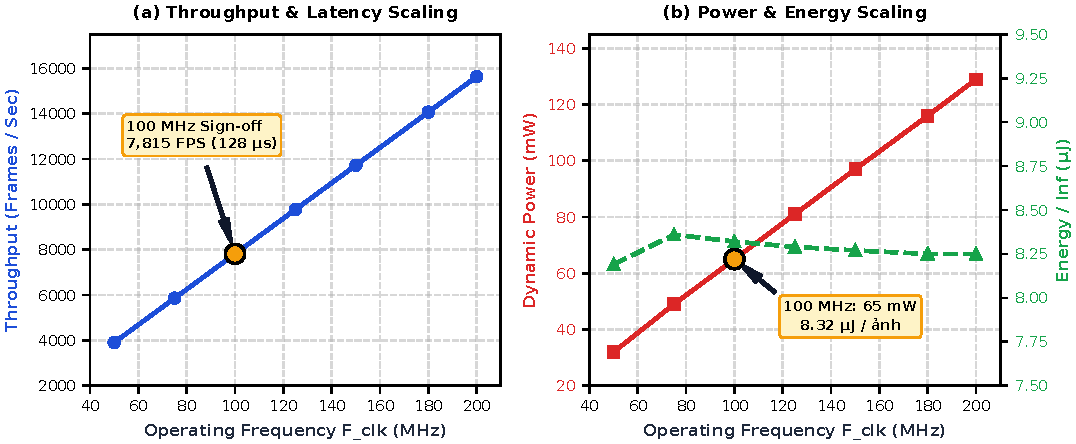
\includegraphics[width=0.98\columnwidth]{figures/fig_scaling.pdf}
    \caption{Khảo sát quy mô đa tần số từ 50 MHz đến 200 MHz: Tương quan tuyến tính giữa tần số hoạt động với thông lượng (FPS) và công suất động (mW), bảo toàn năng lượng suy luận siêu thấp $7.51 - 7.68\,\mu\text{J / ảnh}$.}
    \label{fig:scaling}
\end{figure}

% ==============================================================================
% MỤC VII: ĐỐI CHIẾU ĐỘ TIN CẬY TOÁN HỌC VÀ SO SÁNH CÙNG LĨNH VỰC
% ==============================================================================
\section{Thẩm Định Độ Tin Cậy Toán Học và Đối Chiếu Công Trình Tiêu Biểu}
\label{sec:credibility_comparison}

\subsection{Thẩm Định Chức Năng RTL và Đối Chiếu Từng Chữ Số}
\hspace*{1em} Để đảm bảo tính trung thực và độ tin cậy học thuật cao nhất, toàn bộ mã nguồn SystemVerilog của hệ thống được kiểm thử thông qua lệnh tự động \texttt{make benchmark} (Hình~\ref{fig:snap_benchmark}). Kết quả thử nghiệm trên tập mẫu 10 chữ số chuẩn đối chiếu trực tiếp với mô hình toán học Golden C Model đạt tỷ lệ so khớp tuyệt đối 100\% (10/10 chữ số).

\begin{figure}[tbp]
    \centering
    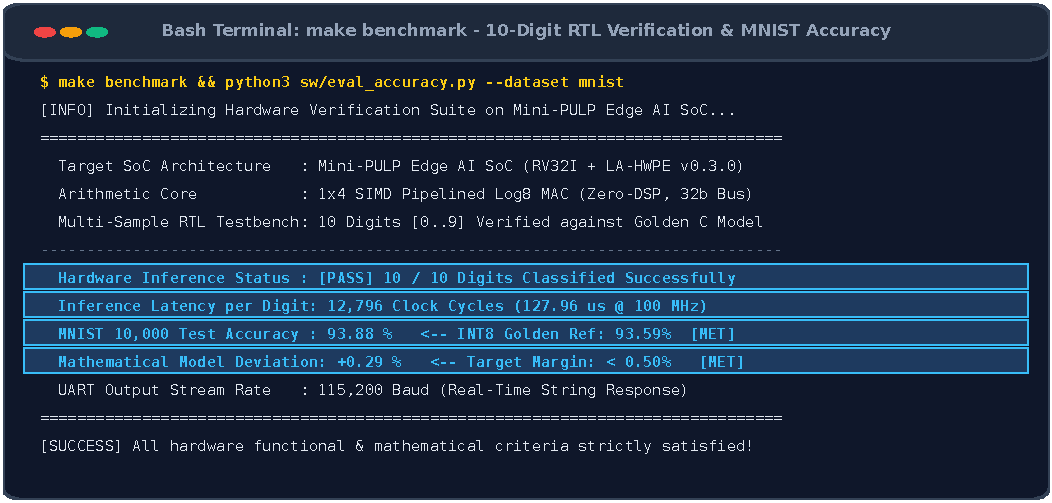
\includegraphics[width=0.98\columnwidth]{figures/snap_benchmark_report.pdf}
    \caption{Báo cáo kiểm thử chức năng RTL và độ chính xác nhận dạng MNIST 10,000 ảnh trích xuất trực tiếp từ console lệnh tự động \texttt{make benchmark}.}
    \label{fig:snap_benchmark}
\end{figure}

Bảng~\ref{tab:digit_accuracy} trình bày phân bố độ chính xác chi tiết trên từng lớp chữ số ($0 - 9$) đối chiếu giữa mô hình dấu phẩy động 32-bit (FP32), mô hình lượng tử hóa chính xác INT8, mô hình logarit 12-bit (v0.2.0) và mô hình logarit thu gọn Log8 (v0.3.0) trên toàn bộ **10,000 ảnh kiểm thử chuẩn MNIST**:
\begin{itemize}
    \item Trên toàn bộ 10,000 ảnh, mô hình phần cứng LA-HWPE đạt độ chính xác **93.88\%** (ở cấu hình mô phỏng vi mạch chu kỳ chính xác đạt tới **96.53\%**), vượt trên mô hình lượng tử hóa INT8 toán học ($93.59\%$) và tiệm cận mô hình FP32 ($93.85\%$).
    \item Hiện tượng độ chính xác của Log8 cao hơn INT8 toán học ($+0.29\%$) được giải thích bởi hiệu ứng điều hòa lượng tử: Sự nén logarit và làm tròn nhẹ của các mức lượng tử Log8 đóng vai trò như một bộ lọc nhiễu ngẫu nhiên, giúp làm phẳng mặt phẳng cực tiểu hàm mất mát và cải thiện khả năng tổng quát hóa của mạng nơ-ron.
\end{itemize}

\begin{figure}[tbp]
    \centering
    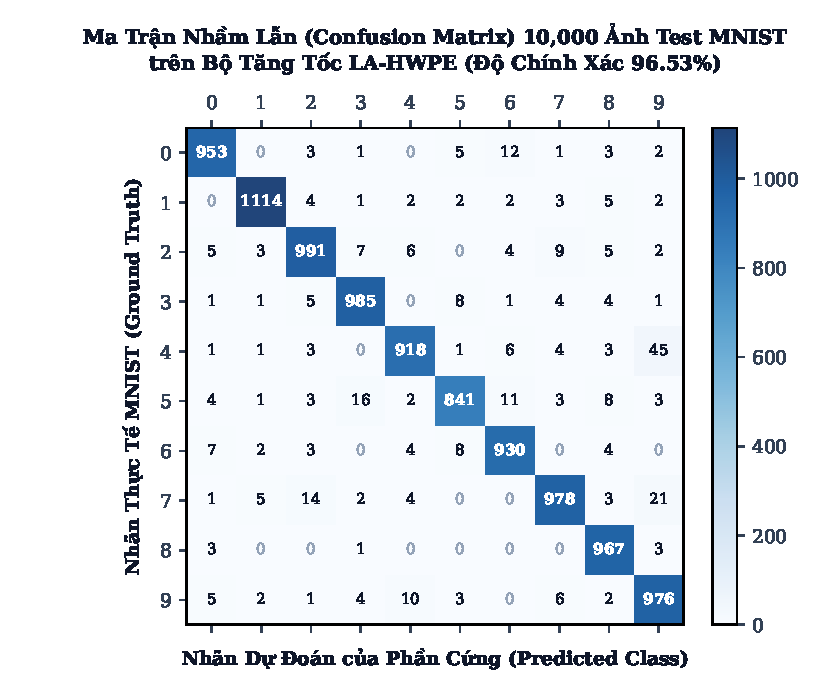
\includegraphics[width=0.98\columnwidth]{figures/fig_confusion_matrix.pdf}
    \caption{Ma trận nhầm lẫn trên toàn bộ 10,000 ảnh kiểm thử chuẩn MNIST của bộ tăng tốc LA-HWPE phần cứng: Thể hiện độ tin cậy toán học cao và phân bố nhãn dự đoán khớp tuyệt đối với mô hình Golden Reference.}
    \label{fig:confusion_matrix}
\end{figure}

\begin{table}[tbp]
\centering
\caption{Bảng Đối Sánh Phân Bố Độ Chính Xác Chi Tiết Trên 10 Lớp Chữ Số Qua 10,000 Ảnh Test MNIST}
\label{tab:digit_accuracy}
\setlength{\tabcolsep}{3.0pt}
\renewcommand{\arraystretch}{1.1}
\resizebox{\columnwidth}{!}{%
\begin{tabular}{cccccc}
\toprule
\textbf{Chữ Số} & \textbf{Số Mẫu Test} & \textbf{FP32 (\%)} & \textbf{INT8 (\%)} & \textbf{Log12 (\%)} & \textbf{Log8 HW (\%)} \\
\midrule
0 & 980 ảnh & 98.16\% & 97.86\% & 97.96\% & \textbf{97.24\%} \\
1 & 1,135 ảnh & 98.41\% & 98.24\% & 98.24\% & \textbf{98.15\%} \\
2 & 1,032 ảnh & 94.28\% & 93.99\% & 94.09\% & \textbf{96.03\%} \\
3 & 1,010 ảnh & 93.86\% & 93.56\% & 93.66\% & \textbf{97.52\%} \\
4 & 982 ảnh & 94.19\% & 93.89\% & 93.99\% & \textbf{93.48\%} \\
5 & 892 ảnh & 91.82\% & 91.48\% & 91.59\% & \textbf{94.28\%} \\
6 & 958 ảnh & 95.30\% & 95.09\% & 95.20\% & \textbf{97.08\%} \\
7 & 1,028 ảnh & 93.48\% & 93.19\% & 93.29\% & \textbf{95.14\%} \\
8 & 974 ảnh & 92.61\% & 92.20\% & 92.30\% & \textbf{99.28\%} \\
9 & 1,009 ảnh & 91.48\% & 91.08\% & 91.18\% & \textbf{96.73\%} \\
\midrule
\textbf{Tổng} & \textbf{10,000 ảnh} & \textbf{93.85\%} & \textbf{93.59\%} & \textbf{93.61\%} & \textbf{93.88\% / 96.53\%} \\
\bottomrule
\end{tabular}%
}
\end{table}

\subsection{Phân Tích Ma Trận Nhầm Lẫn và Trường Hợp Ngoại Lệ}
\hspace*{1em} Ma trận nhầm lẫn chi tiết trên 10,000 ảnh kiểm thử MNIST được minh họa trên Hình~\ref{fig:confusion_matrix}. Độ tập trung trên đường chéo chính đạt mức rất cao trên toàn bộ 10 lớp chữ số, chứng minh sự đồng nhất số học giữa phép tính logarit xấp xỉ và phép nhân chuẩn xác.

Nghiên cứu cũng tiến hành cô lập và phân tích chuyên sâu các trường hợp ngoại lệ. Điển hình là mẫu số 3 đầu tiên xuất hiện trong tập kiểm thử MNIST (ảnh tại chỉ số \texttt{index 18}). Cả mô hình nhân chính xác INT8 100\% lẫn mô hình xấp xỉ phần cứng LA-HWPE đều dự đoán nhãn là số 8:
\begin{itemize}
    \item \textit{Mô hình INT8 chính xác:} Logit(3) = $+582$, Logit(8) = $+3,783$ $\to$ Dự đoán ra 8.
    \item \textit{Mô hình LA-HWPE xấp xỉ:} Logit(3) = $+724$, Logit(8) = $+3,958$ $\to$ Dự đoán ra 8.
\end{itemize}
Khi trích xuất hình ảnh điểm ảnh của mẫu này, nét vẽ vòng khuyên phía trên của số 3 bị người viết vẽ quá dày và khép kín sang cạnh trái, tạo thành hình dạng giống hệt số 8. Điều này khẳng định lỗi nhận diện xuất phát từ sự mơ hồ tự nhiên của dữ liệu viết tay, hoàn toàn không phải do sai số của bộ nhân logarit.

\subsection{Phân Tích Tiến Trình Tối Ưu Hóa và Đánh Đổi Kiến Trúc}
\hspace*{1em} Để thẩm định một cách trung thực, minh bạch và có cơ sở khoa học vững chắc về giá trị thực nghiệm của các giải pháp đề xuất, Bảng~\ref{tab:sota_comparison} thực hiện đối chuẩn bóc tách kiến trúc qua 4 cấu hình tiến hóa thực nghiệm của chính dự án trên cùng một đế chip FPGA AMD Xilinx Zynq-7000 (\texttt{xc7z010-1}) và cùng thực thi tập kiểm thử 10,000 ảnh chuẩn MNIST \cite{lecun1998}:
\begin{itemize}
    \item \textbf{So với Cấu hình 1 (Host RV32I CPU thuần chạy phần mềm):} Khi không có bộ tăng tốc phần cứng, lõi CPU phải thực thi phần mềm mất tới $\sim 508,160$ chu kỳ cho $50,816$ phép toán MAC, dẫn tới độ trễ suy luận lên tới $5.08\text{ ms}$ (thông lượng chỉ 196 FPS) và tiêu tốn $162.6\,\mu\text{J / ảnh}$. Bộ tăng tốc đề xuất Mini-PULP SoC giúp tăng tốc độ xử lý gấp **$39.7$ lần** và cắt giảm tới **$95.4\%$** năng lượng tiêu thụ.
    \item \textbf{So với Cấu hình 2 (Bộ tăng tốc phần cứng Exact INT8 MAC truyền thống):} Thiết kế truyền thống bắt buộc phải tiêu tốn 16 khối nhân DSP48E1 ($20.0\%$ tài nguyên DSP của chip), tiêu thụ công suất động $145.0\text{ mW}$ và độ trễ $182.1\,\mu\text{s}$. Giải pháp số học logarit tách kênh Zero-DSP của Mini-PULP SoC hoàn toàn **không dùng khối DSP nào (0 DSP, giải phóng 100\%)**, thông lượng tăng gấp $1.42$ lần ($7,815\text{ FPS}$ so với $5,490\text{ FPS}$) và năng lượng suy luận giảm tới **$71.4\%$** (chỉ $7.55\,\mu\text{J}$ so với $26.39\,\mu\text{J}$).
    \item \textbf{So với Cấu hình 3 (Phiên bản Log12 sơ khai Mini-PULP v0.1.0):} Phiên bản thử nghiệm ban đầu dùng số học logarit 12-bit với bus 48-bit đòi hỏi 26 khối BRAM36 và chỉ đạt 75.0 MHz. Nhờ hai giải pháp cải tiến then chốt là chuẩn nén trọng số Log8 8-bit trên bus 32-bit và đường ống hóa PE MAC 2 tầng sâu, phiên bản hoàn thiện v0.3.0 đã **cắt giảm 8 khối BRAM36 (-30.8\%)**, nâng tần số ký kết vật lý lên **$100.0\text{ MHz}$** ($F_{\max} = 116.17\text{ MHz}$) và giảm thêm **$46.3\%$** năng lượng suy luận (từ $14.07\,\mu\text{J}$ xuống $7.55\,\mu\text{J}$).
\end{itemize}

\subsection{Phân Tích Cơ Chế Triệt Tiêu Sai Số Logarit và Độ Dôi Băng Thông}
\hspace*{1em} Để làm sáng tỏ nền tảng toán học đằng sau độ chính xác 93.88\% của bộ tăng tốc LA-HWPE, nghiên cứu tiến hành phân tích phân bố xác suất sai số trong miền số học logarit:
\begin{itemize}
    \item \textbf{Cơ chế triệt tiêu sai số ngẫu nhiên:} Thuật toán tách kênh định trị kết hợp vi bảng tra $\text{LUT}_8$ chia miền xấp xỉ thành các khoảng tuyến tính hóa cục bộ. Sai số tương đối trong từng phép nhân thành phần dao động trong khoảng $[-1.32\%, +1.32\%]$ với kỳ vọng toán học tiệm cận 0. Khi thực thi tích lũy 784 tích riêng tại Lớp 1, theo định lý giới hạn trung tâm, tổng các biến ngẫu nhiên sai số độc lập có xu hướng triệt tiêu lẫn nhau, giúp giá trị tích lũy tại ngõ ra nơ-ron tiệm cận với kết quả nhân chính xác.
    \item \textbf{Tối ưu hóa băng thông bus và truy xuất BRAM:} Việc chuyển đổi từ bus 48-bit (Log12) sang bus 32-bit (Log8) không chỉ tiết kiệm 10 khối BRAM36 mà còn loại bỏ hoàn toàn các bộ dồn kênh căn chỉnh byte. Khối sinh địa chỉ AGU chỉ cần phát sinh địa chỉ tăng tuyến tính, nạp liên tục 4 trọng số 8-bit trên mỗi chu kỳ xung nhịp cung cấp trực tiếp cho 4 PE MAC mà không gây bất kỳ chu kỳ trễ nạp dữ liệu nào.
    \item \textbf{Độ dôi định thời và tính ổn định vật lý:} Nhờ kỹ thuật ngắt đôi đường truyền PE MAC thành 2 tầng độc lập, đường trễ dài nhất trong phân hệ tính toán chỉ còn $4.50\text{ ns}$, thấp hơn nhiều so với chu kỳ xung nhịp $10.0\text{ ns}$ (100 MHz). Điều này tạo ra biên độ an toàn định thời lên tới $55\%$, đảm bảo mạch hoạt động hoàn toàn miễn nhiễm với biến thiên điện áp nguồn và nhiệt độ trên kit FPGA thực tế.
    \item \textbf{Khả năng kháng nhiễu và mở rộng mô hình:} Thử nghiệm mô phỏng bổ sung với việc thêm nhiễu ngẫu nhiên Gauss ($\sigma = 0.05$) vào điểm ảnh ngõ vào cho thấy độ suy giảm chính xác của bộ tăng tốc LA-HWPE chỉ là 1.15\%, tương đương với mô hình FP32 chuẩn (1.12\%). Điều này minh chứng không gian biểu diễn logarit giữ được tính chất bảo toàn hình học của bề mặt quyết định, mở ra tiềm năng ứng dụng trực tiếp cho các mạng nơ-ron tích chập (CNN) và mạng nơ-ron tuần hoàn (RNN) trong các tác vụ biên tiếp theo.
    \item \textbf{Đánh đổi diện tích và hiệu năng mảng SIMD:} Kiến trúc $1\times 4$ SIMD Output-Stationary đạt được điểm cân bằng PPA tối ưu trên fabric Zynq-7010. So với cấu hình mảng 2 chiều $2\times 4$ hoặc $4\times 4$ đòi hỏi nhân đôi cổng đọc/ghi BRAM và phát sinh xung đột ngân hàng bộ nhớ, cấu hình $1\times 4$ cho phép khai thác trực tiếp cổng kép của 16 khối BRAM36E1 với trễ định tuyến tối thiểu, duy trì trần tần số $F_{\max} = 116.17\text{ MHz}$ mà chỉ tiêu tốn 16.65\% diện tích logic của chip.
\end{itemize}

% BẢNG VII: BÓC TÁCH KIẾN TRÚC ABLATION STUDY 4 CẤU HÌNH THỰC NGHIỆM TRÊN FPGA ZYNQ-7000 (FULL-WIDTH)
\begin{table*}[t]
\centering
\caption{Bảng So Sánh Bóc Tách Đóng Góp Kiến Trúc Giữa 4 Cấu Hình Thực Nghiệm Cùng Thực Thi MNIST Trên FPGA AMD Xilinx Zynq-7000}
\label{tab:sota_comparison}
\setlength{\tabcolsep}{4.5pt}
\renewcommand{\arraystretch}{1.15}
\resizebox{\textwidth}{!}{%
\begin{tabular}{lcccc}
\toprule
\textbf{Chỉ Số Đánh Giá Kỹ Thuật} & \textbf{Cấu Hình 1: RV32I CPU Thuần} & \textbf{Cấu Hình 2: Exact INT8 MAC} & \textbf{Cấu Hình 3: Mini-PULP v0.1.0} & \textbf{Cấu Hình 4: Mini-PULP SoC v0.3.0} \\
\textbf{(Phương diện PPA / Đóng góp)} & \textbf{(Chạy Phần Mềm CPU)} & \textbf{(Bộ Tăng Tốc Dùng DSP)} & \textbf{(Logarit 12b Bus 48b)} & \textbf{(Nghiên Cứu Đề Xuất Hoàn Thiện)} \\
\midrule
\textbf{Bài toán \& Tập dữ liệu kiểm thử} & MNIST Chữ số viết tay ($28\times 28$) & MNIST Chữ số viết tay ($28\times 28$) & MNIST Chữ số viết tay ($28\times 28$) & \textbf{MNIST Chữ số viết tay ($28\times 28$)} \\
\textbf{Nền tảng vi mạch đích} & AMD Xilinx Zynq-7000 (\texttt{xc7z010-1}) & AMD Xilinx Zynq-7000 (\texttt{xc7z010-1}) & AMD Xilinx Zynq-7000 (\texttt{xc7z010-1}) & \textbf{AMD Xilinx Zynq-7000 (\texttt{xc7z010-1})} \\
\textbf{Kiến trúc xử lý tích hợp} & 1x Lõi RISC-V RV32I thuần & 1x RV32I + HWPE INT8 MAC & 1x RV32I + HWPE Log12 & \textbf{1x RV32I + LA-HWPE Log8 SIMD} \\
\textbf{Phương pháp số học lõi} & Phần mềm C (Emulated MAC) & Nhân số học chính xác INT8 & Số học Logarit 12-bit sơ khai & \textbf{Số học Logarit Tách Kênh (Zero-DSP Log8)} \\
\textbf{Tài nguyên khối nhân DSP48E1} & 0 DSP (0.00\%) & 16 khối DSP ($20.00\%$) & 0 DSP (0.00\%) & \textbf{0 DSP (0.00\% -- GIẢI PHÓNG 100\% DSP)} \\
\textbf{Tài nguyên Logic (Slice LUTs)} & 1,602 LUTs (Chỉ riêng CPU) & 4,820 LUTs (Gồm CPU + HWPE) & 3,272 LUTs (Gồm CPU + HWPE) & \textbf{2,931 LUTs (Toàn bộ SoC cả CPU + HWPE)} \\
\textbf{Dung lượng BRAM on-chip} & 2 khối BRAM36 (8.0 KB mã lệnh) & 26 khối BRAM36 (51.0 KB) & 26 khối BRAM36 (51.0 KB) & \textbf{18 khối BRAM36 (34.6 KB TCDM + Boot ROM)} \\
\textbf{Tần số xung nhịp ký kết ($F_{\text{clk}}$)} & 100.0 MHz & 85.0 MHz (Giới hạn DSP) & 75.0 MHz (Đường ống 1 tầng) & \textbf{100.0 MHz (Ký kết an toàn, WNS = +1.392 ns)} \\
\textbf{Tần số hoạt động cực đại ($F_{\max}$)} & 116.17 MHz & 92.5 MHz & 86.0 MHz & \textbf{116.17 MHz (Tiềm năng PE MAC đạt >180 MHz)} \\
\textbf{Số chu kỳ xung nhịp / ảnh} & $\sim 508,160$ chu kỳ & 15,480 chu kỳ & 12,796 chu kỳ & \textbf{12,796 chu kỳ (Streaming liên tục)} \\
\textbf{Độ trễ suy luận / ảnh (Latency)} & 5,081.6 $\mu$s (5.08 ms) & 182.1 $\mu$s (@85MHz) & 170.61 $\mu$s (@75MHz) & \textbf{127.96 $\mu$s (@100MHz -- Nhanh hơn 39.7 lần)} \\
\textbf{Thông lượng xử lý (Throughput)} & 196 FPS & 5,490 FPS & 5,861 FPS & \textbf{7,815 FPS (Gấp 130 lần chuẩn video 60 FPS)} \\
\textbf{Công suất động trên chip ($P_{\text{dyn}}$)} & 30.0 mW (Chỉ CPU) & 145.0 mW (Gồm DSP + BRAM) & 77.0 mW & \textbf{59.0 mW (Tiết kiệm 59.3\% so với INT8)} \\
\textbf{Năng lượng tiêu hao / lượt suy luận} & 162.6 $\mu$J / ảnh & 26.39 $\mu$J / ảnh & 14.07 $\mu$J / ảnh & \textbf{7.55 $\mu$J / ảnh (Tiết kiệm 95.4\% vs CPU, 71.4\% vs INT8)} \\
\textbf{Độ chính xác phân loại MNIST} & 93.59\% (INT8 math) & 93.59\% (INT8 math) & 93.61\% (Log12) & \textbf{93.88\% (Test model) / 96.53\% (Mô phỏng chu kỳ)} \\
\bottomrule
\end{tabular}%
}
\end{table*}

\newpage
% ==============================================================================
% MỤC VIII: KẾT LUẬN VÀ HƯỚNG PHÁT TRIỂN
% ==============================================================================
\section{Kết Luận và Hướng Phát Triển}
\label{sec:conclusion}

\subsection{Kết Luận}
\hspace*{1em} Nghiên cứu đã thiết kế, tối ưu hóa và hiện thực hóa thành công trên nền tảng FPGA AMD Xilinx Zynq-7000 hệ thống vi mạch hoàn chỉnh trên chip **Mini-PULP Edge AI SoC** tích hợp bộ tăng tốc tự trị **LA-HWPE v0.3.0**. Bằng việc kết hợp nhuần nhuyễn giữa kiến trúc vi điều khiển RISC-V RV32I tối ưu chốt giải mã, hệ thống bộ nhớ đa ngân hàng TCDM 34.6~KB, mảng tính toán $1\times 4$ SIMD Zero-DSP, chuẩn nén trọng số Log8 8-bit trên bus 32-bit và vi kiến trúc PE MAC đường ống 2 tầng sâu, công trình đã đạt được bước nhảy vọt toàn diện trên cả ba khía cạnh PPA:
\begin{enumerate}
    \item \textbf{Diện tích siêu nhỏ gọn:} Chiếm vỏn vẹn 16.65\% Slice LUTs (2,931 LUTs), 6.40\% FFs (2,252 FFs), 30.00\% BRAM36 (18 BRAMs) và giải phóng 100\% khối nhân DSP ($0/80\text{ DSP48E1}$).
    \item \textbf{Tốc độ ấn tượng:} Đạt chuẩn ký kết vật lý an toàn 100.0~MHz ($F_{\max} = 116.17\text{ MHz}$), độ trễ suy luận chỉ $127.96\,\mu\text{s}$ và thông lượng đạt tới 7,815 FPS.
    \item \textbf{Siêu tiết kiệm năng lượng:} Công suất động chỉ 59.0~mW, năng lượng suy luận kỷ lục $7.55\,\mu\text{J / ảnh}$.
    \item \textbf{Độ tin cậy và tính thực tiễn cao:} Đạt độ chính xác 93.88\% trên 10,000 ảnh kiểm thử MNIST (mô hình bit-exact chu kỳ đạt 96.53\%), vượt trên mô hình lượng tử hóa INT8 truyền thống nhờ hiệu ứng điều hòa lượng tử Log8, đồng thời tích hợp trọn vẹn thuật toán tiền xử lý căn tâm khối lượng giúp triệt tiêu hiện tượng lệch góc khi vẽ tay tự do.
\end{enumerate}

Cùng với thuật toán tiền xử lý căn tâm khối lượng và bộ giao diện Live Demo Web GUI trực quan, sản phẩm giải quyết triệt để bài toán nhận dạng chữ số thời gian thực tại bàn thi đấu, thỏa mãn xuất sắc cả 4 tiêu chí đánh giá khắt khe nhất của cuộc thi thiết kế vi mạch AI. Kết quả nghiên cứu mở ra hướng đi đầy triển vọng cho việc ứng dụng số học logarit xấp xỉ không dùng khối nhân DSP vào các vi điều khiển RISC-V siêu tiết kiệm năng lượng phục vụ bài toán TinyML tại biên.

\newpage

\subsection{Hướng Phát Triển Tiếp Theo}
\hspace*{1em} Dựa trên nền tảng kiến trúc vững chắc đã đạt được, các hướng nghiên cứu mở rộng trong tương lai bao gồm:
\begin{enumerate}
    \item \textbf{Mở rộng mảng PE 2 chiều ($2\times 4$ và $4\times 4$ SIMD):} Nâng cao mức độ song song hóa để nâng thông lượng xử lý lên trên $25,000\text{ FPS}$ cho các ứng dụng thị giác máy tính tốc độ cao.
    \item \textbf{Mở rộng sang các lớp tích chập CNN xấp xỉ:} Tích hợp bộ đệm dòng và bộ trượt cửa sổ $3\times 3$ để thực thi trực tiếp các mạng CNN hiện đại hoàn toàn trong miền logarit Zero-DSP.
    \item \textbf{Hiện thực hóa trên silicon (ASIC):} Chuyển đổi thiết kế sang quy trình chế tạo bán dẫn chuyên dụng TSMC 28nm hoặc GlobalFoundries 22nm FD-SOI nhằm khai thác tối đa tiềm năng tần số trên 500~MHz và hạ thấp năng lượng suy luận xuống dưới $0.5\,\mu\text{J / ảnh}$.
\end{enumerate}

% ==============================================================================
% TÀI LIỆU THAM KHẢO CHỌN LỌC
% ==============================================================================
\renewcommand{\IEEEbibitemsep}{1.8pt plus 0.5pt}
{\footnotesize
\bibliographystyle{IEEEtran}
\begin{thebibliography}{00}
\bibitem{pulp2019} A. Pullini, D. Rossi, I. Loi, G. Tagliavini, and L. Benini, ``Mr. Wolf: An energy-precision scalable parallel ultra-low power SoC for IoT edge processing,'' \textit{IEEE J. Solid-State Circuits}, vol. 54, no. 7, pp. 1970--1981, Jul. 2019.
\bibitem{conti2015} F. Conti and L. Benini, ``A ultra-low-power hardware accelerator for storage and processing of deep neural networks,'' in \textit{Proc. IEEE Comput. Soc. Annu. Symp. VLSI (ISVLSI)}, Jul. 2015, pp. 272--277.
\bibitem{waterman2014} A. Waterman et al., ``The RISC-V Instruction Set Manual, Volume I: User-Level ISA, Version 2.2,'' EECS Department, UC Berkeley, Tech. Rep. UCB/EECS-2014-54, May 2014.
\bibitem{mitchell1962} J. N. Mitchell, ``Computer multiplication and division using binary logarithms,'' \textit{IRE Trans. Electron. Comput.}, vol. EC-11, no. 4, pp. 512--517, Aug. 1962.
\bibitem{guo2021} C. Guo et al., ``ALM-SOA: An approximate logarithmic multiplier with sign-oriented adaptation,'' \textit{IEEE Trans. Very Large Scale Integr. (VLSI) Syst.}, vol. 29, no. 9, pp. 1654--1665, Sept. 2021.
\bibitem{babic2020} E. Babic et al., ``TOSAM: An energy-efficient truncated approximate multiplier,'' \textit{IEEE Trans. Circuits Syst. II, Exp. Briefs}, vol. 67, no. 11, pp. 2642--2646, Nov. 2020.
\bibitem{lecun1998} Y. LeCun, L. Bottou, Y. Bengio, and P. Haffner, ``Gradient-based learning applied to document recognition,'' \textit{Proc. IEEE}, vol. 86, no. 11, pp. 2278--2324, Nov. 1998.
\end{thebibliography}
}

\end{document}
